% Copyright (c) 2008-2009 solvethis
% Copyright (c) 2010-2016,2018-2019 Casper Ti. Vector
% Public domain.
%
% 使用前请先仔细阅读 pkuthss 和 biblatex-caspervector 的文档,
% 特别是其中的 FAQ 部分和用红色强调的部分。
% 两者可在终端/命令提示符中用
%   texdoc pkuthss
%   texdoc biblatex-caspervector
% 调出。

\documentclass[openany, UTF8]{pkuthss}
% 如果的确须要使脚注按页编号的话,可以去掉后面 footmisc 包的注释。
%\documentclass[openany, UTF8]{pkuthss}是单页打印
%\usepackage[perpage]{footmisc}

% 使用 biblatex 排版参考文献,并规定其格式(详见 biblatex-caspervector 的文档)。
% 这里按照西文文献在前,中文文献在后排序(“sorting = ecnyt”);
% 若须按照中文文献在前,西文文献在后排序,请设置“sorting = cenyt”;
% 若须按照引用顺序排序,请设置“sorting = none”。
% 若须在排序中实现更复杂的需求,请参考 biblatex-caspervector 的文档。
\usepackage[backend = biber, style = caspervector, utf8, sorting=none, doi=true]{biblatex}
\usepackage{hyperref}
\hypersetup{colorlinks=true,linkcolor=black,
	filecolor=black,      
	urlcolor=blue,
citecolor=black}
\usepackage{listings}
\usepackage{xcolor}
\usepackage{algorithm}  
\usepackage{algorithmicx}  
\usepackage{algpseudocode}  
\usepackage{amsmath}  
\usepackage{booktabs}
\usepackage{multirow}
\floatname{algorithm}{算法}  
\renewcommand{\algorithmicrequire}{\textbf{输入}}  
\renewcommand{\algorithmicensure}{\textbf{输出}}  
\renewcommand{\algorithmicrepeat}{\textbf{循环}}  
\renewcommand{\algorithmicuntil}{\textbf{直至}}  
\renewcommand{\algorithmicreturn}{\textbf{返回}}  
\renewcommand{\algorithmicif}{\textbf{判断条件}} 
\renewcommand{\algorithmicthen}{\textbf{则}} 
\renewcommand{\algorithmicend}{\textbf{结束}} 
\definecolor{codegreen}{rgb}{0,0.6,0}
\definecolor{codegray}{rgb}{0.5,0.5,0.5}
\definecolor{codepurple}{rgb}{0.58,0,0.82}
\definecolor{backcolour}{rgb}{0.95,0.95,0.92}
\colorlet{punct}{red!60!black}
\definecolor{background}{rgb}{1,1,1}
\definecolor{delim}{RGB}{20,105,176}
\colorlet{numb}{black}

\lstdefinestyle{mystyle}{
	backgroundcolor=\color{background},   
	commentstyle=\color{black},
	keywordstyle=\color{black},
	numberstyle=\tiny\color{codegray},
	stringstyle=\color{codepurple},
	basicstyle=\normalfont\ttfamily,
	breakatwhitespace=false,         
	breaklines=true,                 
	captionpos=b,                    
	keepspaces=true,                 
	numbers=left,                    
	numbersep=8pt,                  
	showspaces=false,                
	showstringspaces=false,
	showtabs=false,                  
	tabsize=2,
		literate=
	*{0}{{{\color{numb}0}}}{1}
	{1}{{{\color{numb}1}}}{1}
	{2}{{{\color{numb}2}}}{1}
	{3}{{{\color{numb}3}}}{1}
	{4}{{{\color{numb}4}}}{1}
	{5}{{{\color{numb}5}}}{1}
	{6}{{{\color{numb}6}}}{1}
	{7}{{{\color{numb}7}}}{1}
	{8}{{{\color{numb}8}}}{1}
	{9}{{{\color{numb}9}}}{1}
	{:}{{{\color{punct}{:}}}}{1}
	{,}{{{\color{punct}{,}}}}{1}
	{\{}{{{\color{delim}{\{}}}}{1}
	{\}}{{{\color{delim}{\}}}}}{1}
	{[}{{{\color{delim}{[}}}}{1}
	{]}{{{\color{delim}{]}}}}{1},
%		breaklines=true,
%	frame=lines
}



\lstdefinelanguage{json}{
	basicstyle=\normalfont\ttfamily,
	numbers=left,
	numberstyle=\scriptsize,
	stepnumber=1,
	numbersep=8pt,
	showstringspaces=false
}

\lstdefinelanguage{yaml}{
 keywords={contexts, weight, frequency, keyword, keywords, contextId, true,context,false,null,y,n},
keywordstyle=\color{darkgray}\bfseries,
identifierstyle=\color{black},
sensitive=false,
%moredelim=[l]{}{:},
comment=[l]{//},
morecomment=[s]{/*}{*/},
commentstyle=\color{black}\ttfamily\bfseries,
stringstyle=\color{black}\ttfamily,
%morestring=[l]{-}{},
morestring=[b]',
morestring=[b]"
}
\lstset{
	style=mystyle,
	inputencoding=utf8,
	escapeinside={\%(*}{*)}
}
% 对于 linespread 值的计算过程有兴趣的同学可以参考 pkuthss.cls。
\renewcommand*{\bibfont}{\zihao{5}\linespread{1.27}\selectfont}
\newcommand{\todo}[1]{\textcolor{red}{#1}}
\newcommand{\draft}[1]{\textcolor{blue}{#1}}
\newcommand{\toolname}{词境}
% 按学校要求设定参考文献列表的段间距。
\setlength{\bibitemsep}{3bp}

% 设定文档的基本信息。
\pkuthssinfo{
	cthesisname = {本科生毕业论文}, ethesisname = {Bachelor Thesis},
	ctitle = {双分辨率词云设计与实例分析}, etitle = {Dual-Resolution Wordles: Design \& Case Study},
	cauthor = {谢李文含},
	eauthor = {Liwenhan Xie},
	studentid = {1600017744},
	date = {二〇二〇年六月},
	school = {元培学院},
	cmajor = {数据科学与大数据分析}, emajor = {Data Science and Big Data Technology},
	direction = {可视化},
	cmentor = {袁晓如\ 研究员}, ementor = {Prof.\ Xiaoru Yuan},
	ckeywords = {文本可视化,词云,多分辨率可视化}, ekeywords = {Text Visualization, Wordle, Multiresolution Visualization}
}
% 载入参考文献数据库(注意不要省略“.bib”)。
\addbibresource{reference.bib}

\usepackage{color}

\begin{document}
	% 以下为正文之前的部分,默认不进行章节编号。
	%\frontmatter
	% 此后到下一 \pagestyle 命令之前不排版页眉或页脚。
	%\pagestyle{empty}
	% 自动生成封面。
	%\maketitle
	% 版权声明。封面要求单面打印,故须新开右页。
	%\cleardoublepage
	%% Copyright (c) 2008-2009 solvethis
% Copyright (c) 2010-2017 Casper Ti. Vector
% All rights reserved.
%
% Redistribution and use in source and binary forms, with or without
% modification, are permitted provided that the following conditions are
% met:
%
% * Redistributions of source code must retain the above copyright notice,
%   this list of conditions and the following disclaimer.
% * Redistributions in binary form must reproduce the above copyright
%   notice, this list of conditions and the following disclaimer in the
%   documentation and/or other materials provided with the distribution.
% * Neither the name of Peking University nor the names of its contributors
%   may be used to endorse or promote products derived from this software
%   without specific prior written permission.
%
% THIS SOFTWARE IS PROVIDED BY THE COPYRIGHT HOLDERS AND CONTRIBUTORS "AS
% IS" AND ANY EXPRESS OR IMPLIED WARRANTIES, INCLUDING, BUT NOT LIMITED TO,
% THE IMPLIED WARRANTIES OF MERCHANTABILITY AND FITNESS FOR A PARTICULAR
% PURPOSE ARE DISCLAIMED. IN NO EVENT SHALL THE COPYRIGHT HOLDER OR
% CONTRIBUTORS BE LIABLE FOR ANY DIRECT, INDIRECT, INCIDENTAL, SPECIAL,
% EXEMPLARY, OR CONSEQUENTIAL DAMAGES (INCLUDING, BUT NOT LIMITED TO,
% PROCUREMENT OF SUBSTITUTE GOODS OR SERVICES; LOSS OF USE, DATA, OR
% PROFITS; OR BUSINESS INTERRUPTION) HOWEVER CAUSED AND ON ANY THEORY OF
% LIABILITY, WHETHER IN CONTRACT, STRICT LIABILITY, OR TORT (INCLUDING
% NEGLIGENCE OR OTHERWISE) ARISING IN ANY WAY OUT OF THE USE OF THIS
% SOFTWARE, EVEN IF ADVISED OF THE POSSIBILITY OF SUCH DAMAGE.

% 此处不用 \specialchap,因为学校要求目录不包括其自己及其之前的内容。
\chapter*{版权声明}
% 综合学校的书面要求及 Word 模版来看,版权声明页不用加页眉、页脚。
\thispagestyle{empty}

任何收存和保管本论文各种版本的单位和个人,
未经本论文作者同意,不得将本论文转借他人,
亦不得随意复制、抄录、拍照或以任何方式传播。
否则一旦引起有碍作者著作权之问题,将可能承担法律责任。

% 若须排版二维码,请将二维码图片重命名为“barcode”,
% 转为合适的图片格式,并放在当前目录下,然后去掉下面 2 行的注释。
%\vfill\noindent
%\includegraphics[height = 5em]{barcode}

% vim:ts=4:sw=4


	% 此后到下一 \pagestyle 命令之前正常排版页眉和页脚。
	\cleardoublepage
	\pagestyle{plain}
	% 重置页码计数器,用大写罗马数字排版此部分页码。
	\setcounter{page}{0}
	\pagenumbering{Roman}
	% 中西文摘要。
	% Copyright (c) 2014,2016 Casper Ti. Vector
% Public domain.

\begin{cabstract}
	
	词云是互联网中的常见文本可视化方法,能以艺术的形式通过关键词呈现文段的概要。然而,由于词云并未提供上下文信息,读者实际上无法判断多义词的具体表意,更难以从支离破碎的词语中构建对语料的整体性理解,不利于对数据的分析。
	
	为了进一步编码上下文信息,提高词云的有效性,我们基于多分辨率显示技术提出了一种全新的可视化形式——双分辨率词云,其具有远看是词云,近看是对应上下文的效果。在该方法中,我们首先设计了一个自适应的布局算法,根据词云各关键词的原始位置限定上下文的布局。其次,利用人视觉系统总体分辨率有限的特性,我们在词云的低频分量上叠加上下文信息的高频分量,进一步增强双分辨率词云对于距离的敏感性。我们还探索了双分辨率词云的参数空间,为用户便捷创制双分辨率词云提供了图形界面。尽管该方法自然地适用于大型显示设备,但我们通过语义缩放的交互形式使之适用于台式显示设备。该可视化方法的有效性通过三个真实案例得到验证。
	
\end{cabstract}

\begin{eabstract}
	The wordle is a common visualization on the Internet to provide an aesthetically pleasing summary for a long text. However, due to an absence of the context in the wordle, it remains challenging for the audience to understand the corpus based on separated words, especially those with multiple semantics.
	
	To address the issue, we present a novel visualization, \textit{Dual-Resolution Wordle}, to directly encode the context on a wordle by means of multi-resolution techniques, leveraging the property of human visual system, where the original wordle is visible at a distance, and the context appears at a closer look. In our approach, we first design an algorithm to adaptively fit the context into the shape constraints of the relevant word. Then we blend the high-pass context layer and the low-pass wordle layer to give a final result. Additionally, we systematically explore the parameter space for such visualization and provide an authoring interface for users to create \textit{Dual-Resolution Wordle} on their own data. Though it is naturally suitable for wall-size display, we also adapt the approach into desktop-device via semantic zooming interaction. We demonstrate the effectiveness of the proposed method through three disparate cases from real-world data.
\end{eabstract}

% vim:ts=4:sw=4

	% 自动生成目录。
	\tableofcontents

	% 以下为正文部分,默认要进行章节编号。
	\mainmatter
	% 各章节。
	\chapter{引言}

\section{信息可视化}
信息可视化是一门建立于人类视觉系统感知特性的基础之上,研究图形化数据表征的跨学科研究领域,主要关注于几类特征鲜明的数据类型,包括多维数据、文本、网络与树型数据、时空数据等。它与计算机图形学、人机交互、心理学等相互交叉,也和统计学、机器学习、数据库系统等相辅相成。通过视觉隐喻以及灵活的人机交互,信息可视化将计算机的算力和人的认知结合在一起,能够发挥出与统计模型、自动化数据挖掘算法等截然不同的分析作用。
\draft{有效在什么地方}

随着大数据时代的深入,数据的产生与传播过程均在不断地加速,信息超载和数据过剩等问题带来巨大挑战。一方面,人们需要分析数据,从数据背后隐藏的信息中挖掘出知识和智慧,以此指导实践;另一方面,人们需要通过一些恰当的方式来与外界交流在数据中的认识和发现。而数据可视化正是应对这两种挑战的有力途径。\draft{举例}



\section{文本可视化}

文本是一种典型的非结构化数据,存在于社交媒体、邮件、文档等与人们日常生活息息相关的场景中,是互联网中最主要的结构类型。文本可视化主要关注于待分析语料所蕴含的语义特征,例如词频、主题、情感、逻辑结构、动态演变等,涉及以下三个方面:(1)文本分析——结合自然语言处理的相应技术,提取文本中的信息作为待可视化的特征。(2)可视化呈现——针对特征选择恰当的视觉编码。(3)人机交互——通过一系列的交互切换不同具有内在关联的视图,动态展现数据的不同层面。

\begin{figure}[htbp]
	\centering
	
\includegraphics[width=\textwidth]{figures/wordle_example.png}
	\caption{词云示例。左:《全宋词》高频词\protect\footnotemark;右:ShapeWordle~\supercite{Wang2020}。}
	\label{fig:wordle_example}
\end{figure}

\footnotetext{宋词缱绻,何处画人间. \url{http://fms.news.cn/swf/2018_sjxw/quansongci}}

词云是文本可视化中的经典方法,通过字号编码词频,以此呈现文本特征(见图~\ref{fig:wordle_example})。它最早可追溯到1976年Milgram对心理地图的研究~\supercite{milgram1976}。进入Web2.0时代后,它广见于网络博客与论坛,用以展示各标签、主题的热度,并衍生出了歌词概览~\supercite{Burch2016}等丰富的应用。词云的可视化手段还能够有效地概括大型文本数据并支持进一步的探索分析。在往届IEEE VAST可视分析挑战赛中,不乏竞赛团队通过利用词云而挖掘到线索的经典案例\draft{(例子文献)}。


\section{本文工作及创新点}
词云因其色彩丰富而设计感十足的外观与简洁易懂的解读方式被大量地运用于文本分析或展示,成为当今最受欢迎的可视化形式之一。然而,它在提供关键词时并未具体给出该词所对应的语境,无法准确反映文本的主体内容。此外,由于一般的词云布局算法以优化整体紧凑程度为主,词语间的邻近程度与其语义毫无关联,读者难以从中梳理出逻辑,构建对词云的整体理解。

\begin{figure}[htbp]
	\centering
	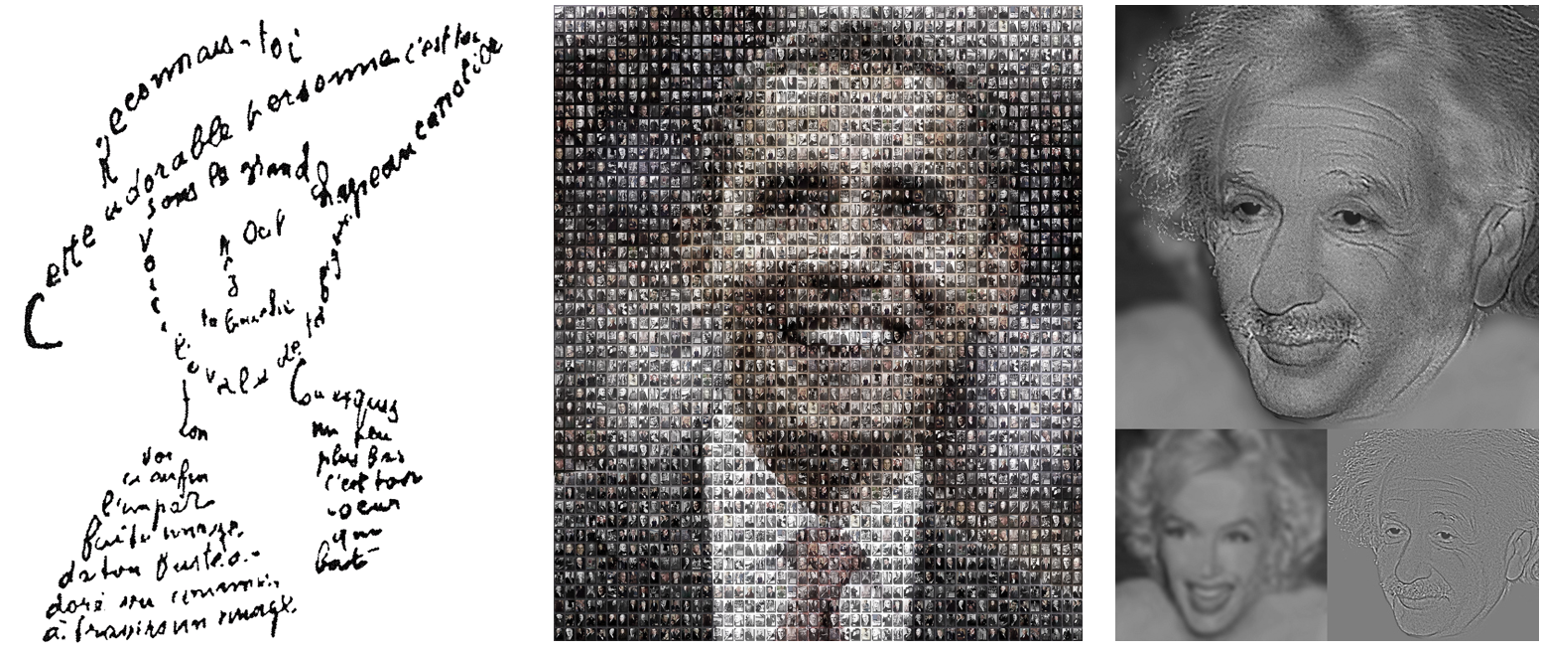
\includegraphics[width=\textwidth]{figures/intro.png}
	\caption{左:图像诗~\supercite{apollinaire1971selected};中:图片马赛克示例;右:混合图像示例~\supercite{Olivia2006}。}
	\label{fig:intro}
\end{figure}


本研究主要是受到多分辨率图像的启发,希望以多分辨率的方式将上下文信息嵌入词云中,在尽可能保留词云美观程度的基础上增加信息的层次,提高词云对文本数据分析的效用,属于一种较为通用的可视化技术。多分辨率图像(示例见图~\ref{fig:intro})在同一图片上用不同编码信息,一般侧重于增强内容的趣味性。例如,法国诗人Guillaume Apollinaire在1915年所开创的图像诗通过精巧的字母布局,将诗句拼凑为相关客体的写意,营造诗与画相谐成趣的效果。又如照片墙常见的的图片马赛克,或者一度引人注目的爱因斯坦与玛丽莲·梦露的混合图像。由于一个关键词往往对应大量的上下文,我们主要考虑在大型显示设备上的双分辨率词云使用场景,以利用其面积大、分辨率高的特性。

本研究的贡献主要包含以下几点:

\begin{itemize}
	\item \textbf{提出了一个新颖的双分辨率词云可视化形式,并设计了相应的生成算法}。这一可视化拓展了词云可视化的设计空间,能够在同一张静态图像上同时编码关键词及上下文信息,弥补现有词云无法提供语境的问题,使分析人员、读者能够更为准确地理解数据,挖掘文本背后的信息。该方法亦可扩展到层次文本数据可视化,具有良好的应用前景。
	
	\item \textbf{基于真实数据构建三个样例,证实了双分辨率词云的有效性}。本研究搜集并整理了《全唐诗》、美国总统特朗普的社交媒体发言以及2020政府工作报告并使用多分辨率词云进行可视化,验证这一方法的有效性。
	
	
	\item \textbf{通过真实案例探究了双分辨率词云的设计空间,实现了一个图形界面以支持用户自定义创制}。对词云布局,目前没有通用的评价准则,且其涉及众多参数,最终结果具有很大的不确定性。为了让用户更好理解参数的意义,我们分析对比了一系列不同参数下的布局结果,并由此给出了一些建议,还提供了一个图形化生成接口支持用户在其他数据上自定义创制双分辨率词云。
	
\end{itemize}

\bigbreak
\bigbreak

\noindent \textbf{文章结构}:本文在第二章介绍相关的感知研究,并对多分辨率技术和词云布局算法进行全面的总结,阐释本研究与现有工作的联系与区别。第三章讨论了多分辨率词云的设计,包括设计目标、设计选择以及早期的实验探索。第四章介绍了本研究提出的双分辨率词云的具体方法。第五章对几个真实数据使用了双分辨率词云可视化,并对其效果进行分析和评价。第六章介绍了协助用户创制双分辨率词云的交互系统。最后,第七章探讨了该研究的应用前景以及未来工作的发展方向。

	% Copyright (c) 2014,2016,2018 Casper Ti. Vector
% Public domain.

\chapter{相关文献}
% vim:ts=4:sw=4
本章对本研究的相关工作进行回顾与讨论,首先是该可视化所依赖的大型显示设备上的相关感知研究,其次是前人在多分辨率技术框架下曾做出的的不同尝试,最后是对该可视化的基础形式词云的综合介绍。

\section{大型显示设备}
\subsection{大屏可视化}
一些工作通过实验证证实了基于大型显示设备(以下简称``大屏'')的可视化的有效性,为我们在大屏上设计多分辨率词云的动机提供了一定的依据。首先,人们能够适应在大屏上高信息密度的数据可视化。Yost和North~\supercite{Yost2006}的定量研究表明,尽管大型高分辨率显示设备展示的信息更多,但用户在大屏完成基础可视分析任务的耗时与小型设备相比没有显著差异。其次,当需要呈现的信息量较多时,用户也相对青睐于视觉信息密度高单一的大屏设置,而不是小屏限制下的的多层渐进可视分析架构~\supercite{Lam2007}。Andrews等人~\supercite{Andrews2010}观察到,大屏所能展示的更多信息为用户检索数据提供了一定的线索,让他们快速获取更多细节,能有效降低他们的记忆负担。最后,大屏也创造了更为丰富的交互空间,包括手势以与物理移动~\supercite{Badam2016} 。大屏自然地提供了一个``聚焦+细节''(Focus + Context)的界面,有利于对数据的探索:用户从远处可看到可视化的整体概览,而稍加移动靠近屏幕时即可观察到特定的细节。这对某些可视分析任务具有独特的优势。例如,当用户需要搜索定位特定区域时,在大屏前的移动会显著快于在常规笔记本显示屏上的鼠标缩放平移~\supercite{Ball2005}。 

\subsection{人对大屏的感知}

我们简要回顾过往相关的实验与研究,以理解在设计大屏双分辨率词云时所需要考虑的因素。
\begin{figure}[htbp]
	\centering
	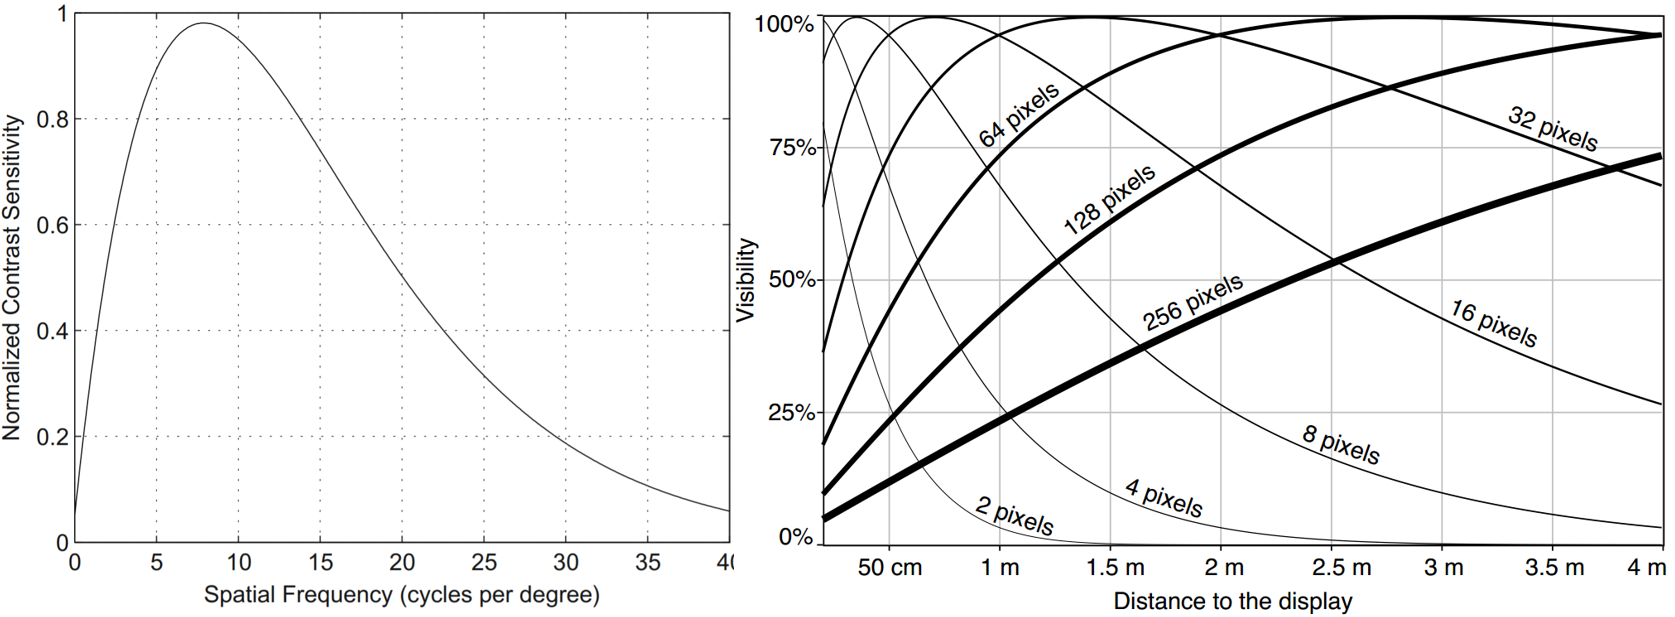
\includegraphics[width=\textwidth]{figures/function.png}
	\caption{左:一个典型的CRF模型~\supercite{Bull2014},横轴为正弦波的空间频域,纵轴为视觉敏感性指标。右:大屏可视范围,横轴为人与显示设备距离,纵轴为可见最小像素~\supercite{Isenberg2013}。}
	\label{fig:function}
\end{figure}

大屏上内容的可分辨性受多种要素影响,如人的视力、视敏度等。一般而言,高对比度的物品会比低对比度的物品更易于分辨。对比-敏感方程~\supercite{Bull2014}(Contrast-Sensibility Function,简称 CRF,见图~\ref{fig:function})拟合了人对不同频率的正弦光栅图的识别阈值的实验结果,反映了视觉神经元对图片对比度的敏感性,表明人的视敏度在3$\sim$4  cpd\footnote{cpd,即cycles per degree,描述视界中正弦光栅图出现的次数,衡量图像特征的空间频率。}时达到峰值,到60 cpd后完全不可见。Isenberg等人~\supercite{Isenberg2013}在大型显示设备~\footnote{该大屏由8×4个30寸显示设备构成,各为2560×1600像素,100ppi。}上用类似的光栅图测试了距离与可见度的关系(见图~\ref{fig:function}),发现不同的特征具有不同的最佳距离,对2或4 ppc的小型特征,它们的可见性在稍近处达到峰值后迅速下降。相反地,对128或256 ppc的大型特征,它们在近处不可见,而到两米外的稍远处维持稳定可见。而对于8$\sim$64 ppc的中等特征,它们具有不同的峰值点与理想可视区域~\footnote{ppc,即pixels per cycle,描述正弦光栅图中一个周期所占像素值。$cpd = \pi / (360tan^{-1}(\frac{p}{2d}ppc))$。}。进一步与普通显示器的对比表明,大屏具有独特的稳定可视距离,而对于一般的显示器而言,只有在60cm处对2$\sim$4 ppc的特征才能达到峰值。这一特性为我们希望人们在不同距离下观察到不同可视化的初始想法提供了可能。

此外,人在大屏上的视觉感知具有一定的局限性。尽管人的视野跨越了170°,但只有以视锥顶点为中心向外张开的20°至40°才是人理想的阅览视角~\supercite{Swaminathan1997}。对于大屏,人们同样倾向于关注40°以内的视野范围,当显示的内容过宽,他们往往会调整自己与屏幕的距离以避免重复的头部移动以及可能的视角扭曲~\supercite{Isenberg2012}。


\section{多分辨率技术}
视觉的产生是因为光线传入视网膜后刺发感光细胞,激发大脑皮层对特定空间频域的并行化处理,由此识别出对应特征。大量心理学研究表明,人的视觉系统对信息的处理具有不同的尺度~\supercite{Joubert2007}。而这种尺度的选择会依人们所需要执行的任务要求发生改变。Olivia和Schyns通过实验发现,在分类任务下,视觉系统会关注于信息量最高的尺度~\supercite{Oliva1997}。本研究所谓的“多分辨率”指的是基于观察者距离界面的不同距离、视角,在同一个静态视图中以不同的分辨率编码信息。以下我们梳理并分析目前我们所知的散见于各学科领域基于多分辨率框架下的工作,探讨他们对多分辨率词云研究的借鉴意义与局限。


\subsection{多分辨率可视化}
多分辨技术能够让观众通过物理位置的变换来动态改变观察视图,因而能够自然地支持信息可视化中奉行的``先概览,通过聚焦和过滤进行筛选,最后提供细节信息''的交互准则~\supercite{Shneiderman96}。然而,目前较少工作利用到了这一技术,主要有频域滤波和图形嵌套方法,该方向尚有很大的研究空间。

\paragraph{频域滤波}Olivia和Schyns~\supercite{Olivia2006}基于他们进行视觉系统信息处理尺度研究实验时所使用的多分辨率技术,在后来综合提出了混合图像的图形学方法,开创了基于频域滤波的多分辨率技术。即通过空间频域滤波,保留远处可见图片A的低频通道,以及近处可见的图片B的高频通道,再利用透明度通道将A与B叠加~\supercite{Baudisch2004},得到同时显示不同细节程度的图片。尽管他们为混合图像构想了四种应用类型,包括揭示同一空间随时间的变迁、动态人像表情、精细纹理混合和文字加密,但他们主要关注于单一或具并列关系的图像,没有考虑编码多层次的信息。特别地,尽管他们从加密的角度特别探讨了文字的多分辨率问题,用随机添加低频噪音的方式防止旁人从远处偷窥文本,但这与我们试图在双重距离范围内使文本清晰可辨大相径庭。此前Majij等人~\supercite{Majaj2002}也在研究字符识别与文字属性(如字体、字号、噪音)的关系时,创造出了同时具有四重分辨率的单字符混合图(见图~\ref{fig:nres}),一定程度上说明了多分辨率方法对字符同样有效。不过,他们着眼于单个字符,而人们对词云的感知是整体性的,还涉及到多文本的共同作用,本研究将更为细致地去考察人们对多分辨率词云的认知感受。

受到混合图像的启发,Isenberg等人\supercite{Isenberg2013}提出了混合图像可视化的概念,指出在大屏上展示静态的混合可视化有助于多人合作可视分析场景。他们在细致分析墙面规模树图、点线图、双刻度散点图与折线图的案例后,进一步探讨了大屏数据可视化中的多分辨率设计准则与任务支持(见图~\ref{fig:nres}),一定程度上说明了多分辨率可视化的广阔应用前景。正是这一工作启发了我们在大屏上同时展示双分辨率下的词云,本研究将在渐进式展现文本数据这一任务的驱动下填补多分辨率词云设计的空白。


\begin{figure}[htbp]
	\centering
	
\includegraphics[width=\textwidth]{figures/nres.png}
	\caption{依距离变化可视层级的多分辨率可视化。左:具有四重分辨率的字符设计,由近及远分别是C、D、E、F~\supercite{Majaj2002};右上:FatFont设计示例~\supercite{Miguel2012};右下:大屏上的多分辨率树图~\supercite{Isenberg2013}。}
	\label{fig:nres}
\end{figure}


\paragraph{嵌套图形}另一个类似于本研究思路的可视化案例还有FatFont~\supercite{Miguel2012}(见图~\ref{fig:nres}),这是一种在半色调(Half-toning)~\supercite{Ostromoukhov1995}的基础上利用特殊字体设计来可视化数值的方法。它通过嵌套的方式将高位数字置于最外层,并用字体粗细编码数值大小,使得从远处看时,特定区域的墨点密度能够反映此处的对应信息,构成点画(Stipling)~\supercite{Gortler2019};从近处看时,准确的数值指标能够直接获取。它对罗马数字进行了再设计,适用于空间型数据的可视化,是对视觉通道~\supercite{Munzner2014}的延伸;而本研究侧重于探索常规排列的字符集,以不同的分辨率编码词云,使其相互作用来辅助文本分析。



\subsection{图形排样}
计算机图形学中的非真实感渲染~\supercite{ThomasStrothotte2002}旨在以计算的方式重现艺术化的表现形式。图形排样属于这一领域的子方向,主要研究以特定图案或纹理样式作为最小单元而构成具有审美性的图形。按照最小单元类型,这种方法可进一步分为基于图案碎片的图像拼接(Mosaicking)与基于字符文本的图像诗(calligram)。

\paragraph{图像拼接}参考Battiato等人的综述~\supercite{Battiato2007},图像拼接的方法主要有两种途径:(1)先分解原始图像,再重建产生特殊碎片效果,如马赛克墙饰;(2)从较大的碎片集合中选取元素拼凑为待拟合的图像。其中,最接近本文的多分辨率词云概念的是后者,特别是一种基于不规则图形的拼图式图像拼接,因为字符是不规则的。一大类算法是采用的是优化的观点。以Jigsaw Image Mosaicking~\supercite{Kim2002}算法为代表,它定义了一个由空隙、颜色、重叠、图样变形综合作用的能量函数,通过最小化基础图形排布引发的开销得到解决方案。类似地,Dalal等人~\supercite{dalal2006}通过最小化距离度量与空隙面积来均衡化基于Voronoi区域的分割。而另一大类方式则是基于搜索。如Blasi等人~\supercite{Gallo2006}先对图片进行分割,再在备选图集中匹配最优碎片并进行图像处理使其接近于背景图像。

\paragraph{文字诗}在涉及文字的自动化排布问题中,总体而言研究的数目比较少,其最终效果也和人为创作的文字诗略有区别。我们归纳出了目前存在的三种方向(见图~\ref{fig:calligram})。

\begin{enumerate}
	\renewcommand{\labelenumi}{(\theenumi)}
	\item 通过扭曲字符来适应形状限制。Zou等人~\supercite{Zou2016}根据指定的形状轮廓计算出文字布局的路径,并在沿路径排列字符后通过特定的指标优化矢量字符控制点的位置,使字符尽可能填充区域并保持可识别。不过,这一方法需要基于大量训练数据来得到衡量变形字符可识别性的损失函数并据此优化,因而难以运用于在中文等字符库巨大的语言。类似的工作还有\parencite{Xu2007,Chi2018}等。
	\item 字符艺术。Xu等人\supercite{Xu2010}以\texttt{Ascii}字符做为图形的``像素'',通过纵横排布,使之尽可能接近原始图像的线描。
	\item 基于区域向量场排布。Moharik等人~\supercite{Moharik2011}计算了外层图形轮廓所张成的向量场,由此生成语料文段排列的路径集合,以此排列大段文字,并通过轻微调整每一行的高度使其更多地填充图形。
\end{enumerate}


\begin{figure}[htbp]
	\centering
	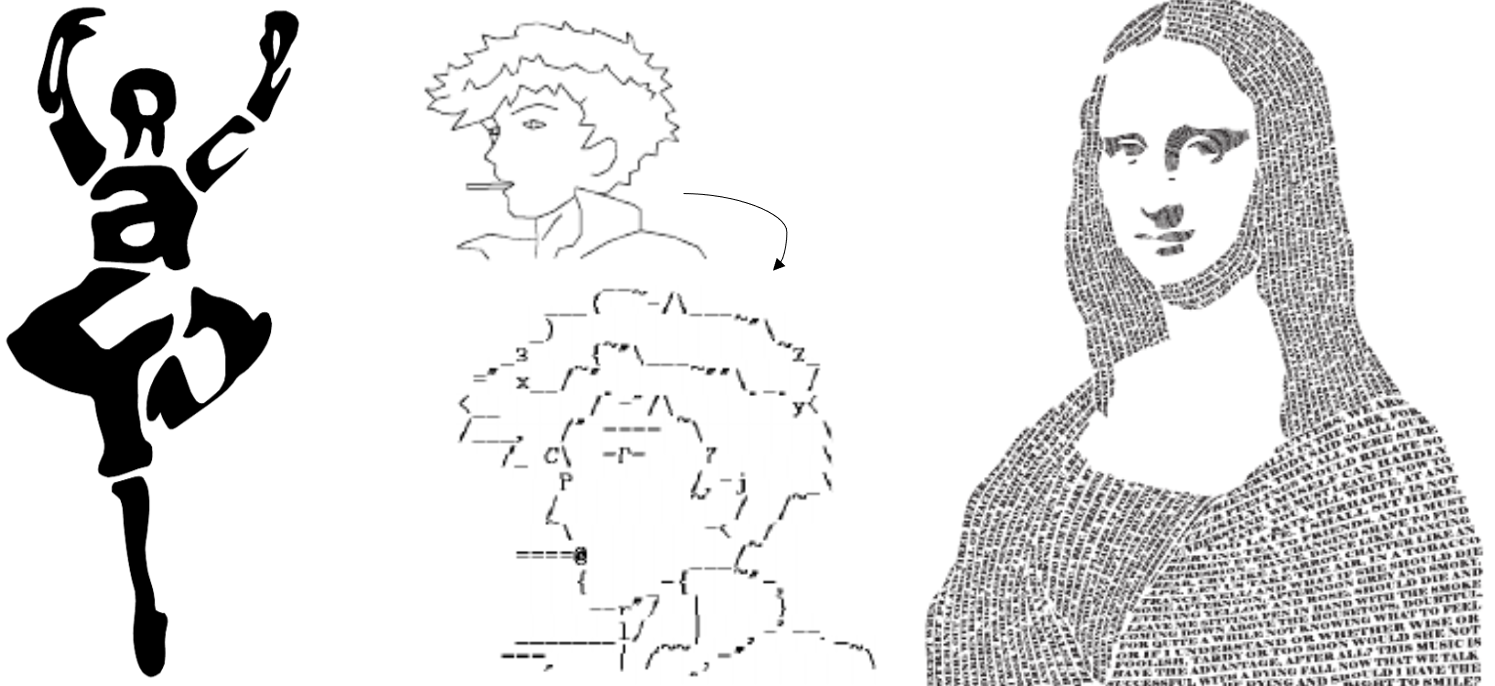
\includegraphics[width=0.8\textwidth]{figures/calligram.png}
	\caption{以字符为基础的文字诗图形排样方法。左:字母变形~\supercite{Zou2016};中:Ascii字符艺术~\supercite{Xu2010};右:文段依向量场排布~\supercite{Moharik2011}。}
	\label{fig:calligram}
\end{figure}

\bigbreak
图形学的相关工作尽管与本文所要探索的内容在最终效果有一定相似之处,但其主要考虑的是在给定图像上的填充,对艺术性及趣味性的要求往往高于文本可读性,有时会根据区域形状对字体样式进行变形,字的大小与位置通常仅与填充的需求相关~\supercite{Kyprianidis13}。而多分辨率词云所依赖的数据为具有双层结构的词集,最终布局是灵活的,且其对于文字的可识别性有更高的要求,需要通过字的大小反映词频等重要性指标,以此辅助完成文本分析任务。在处理上下层词云的布局关系时,我们在一定程度上借鉴了图像拼接的基本思路,例如先分割再排布、对区域进行预处理等等。而对于词云这一特殊可视化的布局,我们进行了更为深入的考量。


\subsection{媒介相关方法}
对于一些具有特殊物理特性的显示媒介来说,人们在不同视角下能够观察到的仅为其整体显示中的局部。在此基础上,人们就可以在同一个媒介中隐藏不同层次的信息。例如,装饰画中常见的光栅立体图~\supercite{Yitzhak2018}就利用了塑料光栅板对光线的折射与衍射,改变图像上各点光线传播的方向,使人的双眼分别观察不同的图片,在视位差的作用产生立体感。类似地,Kim等人注意到了扭曲向列型液晶显示屏(TN-LCD)在不同观察角度下对应的颜色亮度不一致。利用这种感知差异,他们通过将两幅图像同时在时间频域与空间频域逐像素交错显示的方法,制造出一系列从不同方位看有不同内容的图片~\supercite{Kim2012}。媒介相关的多分辨率技术巧妙地借助了显示硬件的物理特性,但受限于此,不利于推广。此外,他们多依赖于观察者视角的切换,因此难以建立起明确的交互语义。相对而言,上文所述的图形排布与嵌套以及频域滤波的方法则是通过观察者与观察对象的距离而改变产生不同的视图,人们在由远及近时具有先概览、后细节的自然交互,因此更适合于可视化。

\bigbreak
需要仔细区分的是,我们所研究的多分辨率技术与缩放有所区别。缩放能改变显示的信息层级,模拟观察距离或语义层次的改变,让用户能够从概览中找出感兴趣的区域再进一步定位~\supercite{Cockburn2009}。但它动态地改变了用户的视图,不利于多人合作的场景,因而不做探讨。在时间序列可视化中,也有“多分辨率”的说法。这指的是在一个视图整体中同时展示不同时间粒度下的聚合信息~\supercite{Hao2007},亦不属本文所研究范畴。

\section{词云}
词云在引言中已有介绍,以下回顾词云的代表性布局算法以及其在文本可视分析中的应用案例。

\subsection{布局算法}
词云的布局算法一直是研究的热点。Viegas等人~\supercite{Viegas2009}最早提出Wordle的概念,突破了传统词云无法旋转、样式单一等局限,具有很强的艺术性。他们在布局时使用的是贪心算法:首先为每一个词语随机设定初始位置,或按照字母序沿横轴均匀排布,或围绕中心发散排布;每当词与词的边界框产生交叠,便沿螺旋线方向相应调整词语位置。而Rolled-out Wordle~\supercite{Strobelt2012}改进了Wordle迭代更新时逐元素检查是否交叠的策略,换以图像逐行扫描或沿圆心放射扫描,以此保证整体布局的紧凑性。不少布局算法还考虑了语义,使关联强的词语聚簇在一起。Cui等人~\supercite{Cui2010}提出了自适应的力导向词云布局算法,先为各大意群随机设定位置,以此为中心初始化词语,再通过引力与斥力的模拟微调布局。Wu等人~\supercite{Wu2011}则是以MDS投影设定各词语初始位置,维护基于语义关联的距离度量,再通过线裁剪去除空白部分。特别地,一部分工作在自动化布局的基础上为设计者提供交互修改的自由度,如支持鼠标选择移动的ManiWordle\supercite{Koh2010}和支持手写笔的WordlePlus~\supercite{Jo2015},以及进一步维护紧凑布局的EdWordle~\supercite{Wang2018}等。

形变词云(Morphable Word Cloud)类似于文字诗,支持用户指定词云外层的轮廓形状,能够产生多分辨率的效果。Chi等人~\supercite{Chi2015}将每个词视为有质量的刚体,通过动力学原理为布局添加边界等限制进行迭代。借助物理模型,他们不仅有效限制了词云的形状,还为展示词云随时间的变化提供了流畅的过渡。ShapeWordle~\supercite{Wang2020}延拓了以往空隙填充算法中使用的螺旋线,通过外层轮廓对应的向量场为词云所在区域重新定义了距离场,使得在迭代过程中词语能以接近外层轮廓的螺旋线调整。

对词云布局的评价标准是多样化的。参考Barth等人~\supercite{Barth2014}的工作,评估一个词云布局算法的优劣可从以下几个角度考虑:(1)布局紧凑性,即是否充分使用空白的区域;(2)布局均匀性,即词云的位置是否足够随机,留下均匀分布的空白区域;(3)维护语义的能力,相似语境下的的词语能否聚到一起。我们无意研究一个新的词云生成算法,而是考虑在现有算法的基础上加入多分辨率技术,使用户可以在不同场景下选择更为合适的基础词云形式。本文在具体实现时主要利用了基于贪心策略的算法,而对细节部分的布局则考虑了一些形状上的限制,第~\ref{sec:refinement}节将具体讨论。

\subsection{文本可视分析}
尽管词云是最易于理解的可视化方法之一,但利用词云完成分析型任务还存在诸多挑战。例如,字号并非编码定量型数据的最佳视觉通道~\supercite{Munzner2014}。对于处于同一级别的词语,尽管它们的字号是一样的,但字数更长的词所占的面积会更大,潜在地影响了人的判断,营造出它更为``关键''的假象;而词语的布局位置与词本身没有明确的对应关系,当用户有特定感兴趣词汇时并难以快速定位搜索~\supercite{Lohmann2009};此外,由于脱离了上下文,人们难以从零星的关键词中构建完整的理解~\supercite{Viegas2008}。近期,Felix等人~\supercite{Felix2018}基于不同的分析任务对比了几种展示关键词的设计选择,认为词云更适合于抽象的文本分析任务,如概括与理解话题,而它对于精确的数据分析任务并非是最有效的。

为了应对以上挑战,一方面,许多布局算法将强关联的词语聚合在相邻区域以增强用户对整体概念的把握和理解,而另一方面,一些可视分析工作结合具体的任务需求,将词云与其他可视化形式有机结合,挖掘交互探索的可能性,使词云综合发挥作用。SentenTree~\supercite{Hu2017}借助自然语言处理中的语义解析技术,用树的形式展现社交媒体中的热门话题及其分支,保留了短语逻辑的完整性。Parallel Word Clouds~\supercite{Collins2009}以词垂直布局作为平行坐标轴对比数据的不同层面。本研究所关注的大屏多分辨率词云属于对大规模词云布局的底层可视化技术,适用于时序语料以及大型非结构化文本数据。在这一主题下,涌现了相当多的工作。SparkClouds~\supercite{Lee2010}将词语与迷你折线图合并为基础布局单元;WordStream~\supercite{Dang2019}以主题河流图的形式展现了关键词的变迁。此外,少数工作探索了大型语料库的渐进性探索。TexTonic~\supercite{Paul2019}借用地图的隐喻,为维基百科这样的大规模文本库提供了用户主导的交互式词云可视化,将原始文本、片段聚类、关键词以多层次地图疆界的方式结合(见图~\ref{fig:textonic})。

\begin{figure}[htbp]
	\centering
	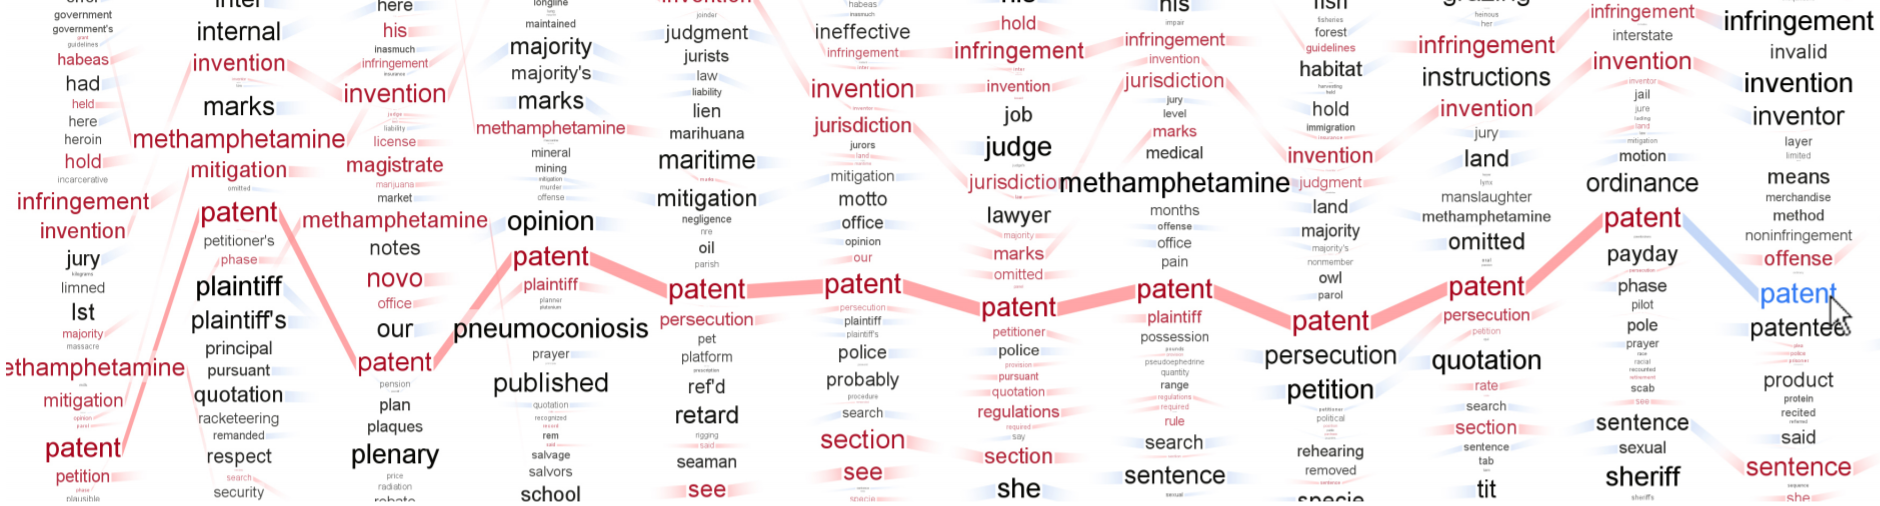
\includegraphics[width=\textwidth]{figures/parallel.png}
	\caption{Parallel Word Clouds~\supercite{Collins2009}:大型时序平行坐标词云。}
	\label{fig:textonic}
\end{figure}

\begin{figure}[htbp]
	\centering
	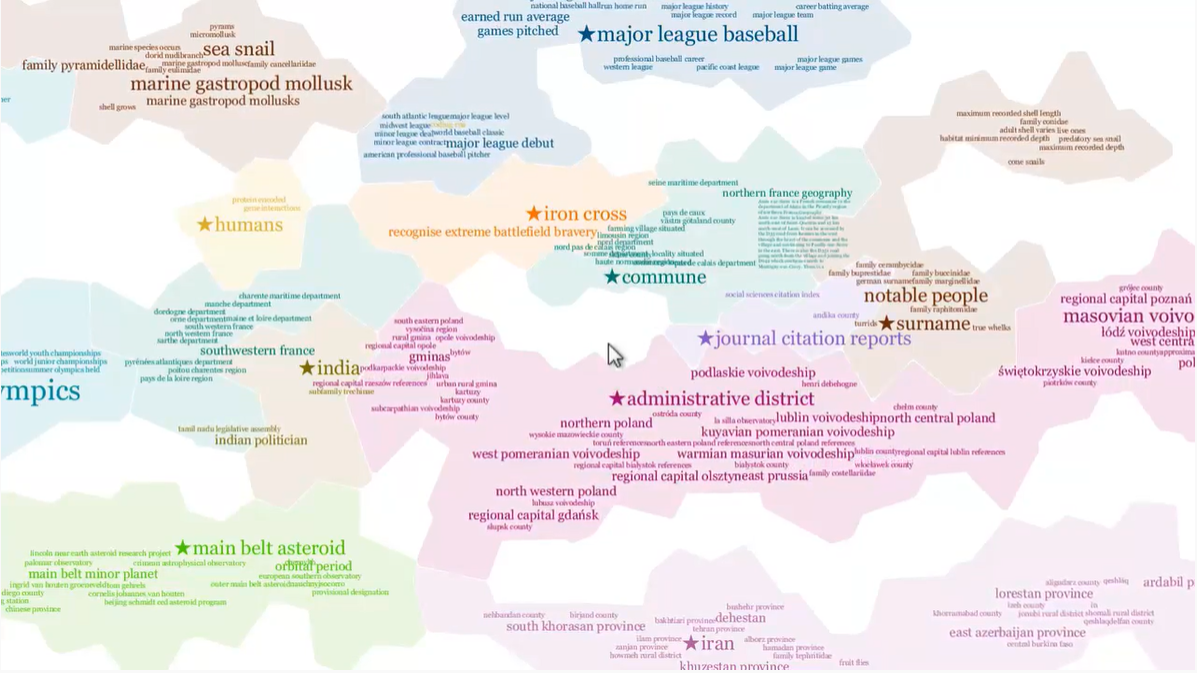
\includegraphics[width=\textwidth]{figures/TexTonic.png}
	\caption{TexTonic~\supercite{Paul2019}:基于地图词云的大型文本交互探索系统。}
	\label{fig:textonic}
\end{figure}

	\chapter{双分辨率词云的设计目标}

为了合理提出双分辨率词云及其自定义创制系统的视觉设计,本章节将讨论双分辨率词云所关注的任务与使用情境,结合可视化中相关的重要设计准则,推导出设计要求,以此在众多首要的设计选择中明确具体的方案,明确设计的方向。

\section{任务}
双分辨率词云是一种通用的文本可视化方法,其核心是延拓现有词云,提供对上下文的支持,在静态图像中额外编码关键词对应的语境。我们认为,无论是出于探索式数据分析的需求还是出于可视化具有关联的文本的需要,双分辨率词云都能发挥一定的作用。此外,无论是词云还是多分辨率图像,他们都能够娱乐观众,兼具艺术性和趣味性。而脱胎于此的双分辨率词云亦应继承这一良好特性。

\begin{enumerate}[leftmargin=*]
	\renewcommand{\labelenumi}{\textbf{T\theenumi.}}
	\renewcommand{\labelenumii}{\textbf{ T\theenumi.\arabic{enumii}}}

	\item \textbf{探索式数据分析}---尽管词云不涉及复杂的自然语言处理技术,仅凭借词频粗略地概括文本内容,但它很适用探索式数据分析的情境。当分析者对数据一无所知,尚未建立任何猜想或假设,关键词这种回归原始数据的底层信息能够使分析者快速构建对数据自身的理解,了解文本中的主要话题。而双分辨率词云则是进一步提供了具体的语境,使得分析者可通过递进的方式进行探索,更为准确地理解数据。
%	他们所关心的问题可能包括
%	\begin{itemize}
%		\item 这一文本有什么内容?
%	\end{itemize}

   \item \textbf{层次化文本数据展示}---双分辨率词云的形式除了能够展示关键词及其上下文,也可用于展示其他具有二重层次关联的文本数据。例如外层词云对应主题,内层词云对应主题下的关键词的情况。它能将抽象的数据处理结果可视化,辅助交流与沟通。

%   在这一任务的驱动下,双分辨率词云应解决
%   \begin{itemize}
%   	\item
%   \end{itemize}
%
   \item \textbf{寓教于乐}---所谓“一图胜千言”,生动的信息图表(Inforgraphics)往往能激发观众的兴趣,带来别样的浏览体验~\supercite{Munzner2014}。我们希望双分辨率词云具有寓教于乐的功能,在反映数据的同时兼具艺术性与趣味性,让随机浏览的人们沉浸其间,使创作者能更好地向大众传达词云所隐含的信息。

\end{enumerate}


\section{设计准则}

除了以上对分析情境及对应任务的考量,我们在双分辨率词云的设计中也需要考虑一些普适的设计准则与认知规律。
\begin{enumerate}[leftmargin=*]
	\renewcommand{\labelenumi}{\textbf{P\theenumi.}}
	\renewcommand{\labelenumii}{\textbf{ P\theenumi.\arabic{enumii}}}
	\item \textbf{可视化设计标准}
		\begin{enumerate}
		\item \textbf{Gestalt理论}---Gestalt理论~\supercite{Wagemans2012ACO}描述了人们在感知或理解图像时,根据某些特征将元素聚集所表现出来的规律。通过这种机制,人们得以简化图像的模式、理解其内涵。其中,与本研究相关的规律有以下三点。
		\begin{itemize}
			\item \textit{相似性聚集}:相似的元素会被视为一类。我们习惯于会不自觉将形状或色彩等基本视觉属性接近的元素划归为一类,认为他们具有相同的作用。
			\item \textit{相邻性聚集}:物理位置上靠近的元素会被视为一类。而对于彼此存在巨大空隙的元素,就算他们在外观上具有一定相似性,我们也倾向于认为他们之间无关。即是说,相邻性聚集的作用远远大于相似性聚集。
			\item \textit{共享空间聚集}:处于同一封闭区域内部的元素会被认为同属一类。
		\end{itemize}
		\item \textbf{自顶而下的探索流程}---可视化领域广泛认可``先概览,通过聚焦和过滤进行筛选,最后提供细节信息''~\supercite{Shneiderman96}的交互探索流程,大量应用均遵循着这一原则。概览让用户首先对数据产生基本的认识,定位到感兴趣的数据子集,再从细节中完成更为精细的分析任务。
		\item \textbf{使用更少的视图。}在具有多个视图的可视化中,应尽可能减少所使用的视图数目~\supercite{Baldonado2000}。尽管利用交互切换视图能帮助用户在数据概览中渐进地定位到关键区域,对更多的细节展开探索,但过多的视图切换伴随着额外的认知开销,会产生学习与交互成本,使用户难以构建对数据的宏观理解(Mental Map),最终影响数据分析的效率。
	\end{enumerate}
	\item \textbf{美观标准}
			\begin{enumerate}
	\item \textbf{空间覆盖率高}---参考Wang等人~\supercite{Wang2020}对词云美观性的评价指标,我们以词云中空白区域像素个数占所有像素个数的比例作为度量。
		\item \textbf{布局均匀}---在词云的布局中,无关联的文本应均匀地布局在图片上。换而言之,词与词之间的空隙是均匀分布的。
		\item \textbf{字符清晰可辨}---两层词云各不影响。在最理想的情形下,对于特定的距离范围,只有父词云或子词云可见,且同级词云均可清晰辨别。
	\end{enumerate}
\end{enumerate}

\section{设计选择}
\paragraph{大屏还是小屏,静态还是交互?}
双分辨率词云的初衷是为基本的词云提供上下文信息,使人们能够结合语境更好地理解数据。以此为出发点,我们其实还有许多设计选择。由于除了客观的人眼感知能力与计算机硬件性能,可视化工具展示数据的能力(即视觉可扩展性\supercite{Eick2002}) 还受到屏幕分辨率、可视系统的交互性、可视化隐喻内涵等因素的影响,我们由此来考虑备选设计。

首先是交互性。在可视分析中,许多系统为用户提供了多种相互关联的视图,让他们通过自行筛选来浏览更多的细节,逐渐发掘数据背后的知识。类似地,我们可以提出这样的一个设计:只显示父词云,再通过动态查询~\supercite{DBLP:journals/software/Schneiderman94}展示相应的子词云信息,如返回一个列表。结合我们的任务,答案是否定的。这种渐进式的探索需要用户确定感兴趣的区域,再去执行筛选而改变视图,缺乏即时性。对于向多人展示的场景(T2),无法体现数据的全貌,缺乏说服力。而对受众随机浏览的场景(T3),由于交互不是显式存在的,极有可能会被忽略,最终与静态普通词云的效果无异,背离了初衷。

而由于文本的非结构化特性,为其换用图形表征是较为困难的,因此不予考虑。最终,我们选择在大屏上静态地同时显示上下层词云。提高屏幕分辨率后极大遍历了大量信息的同时显示。在现有的任务框架下,针对大屏的静态可视化设计是最佳选择。借助引人入胜的多分辨率技术(T3),其只需要一个视图(P1.3),较易使人理解。人们在远处即可获得对整体的认知,确定感兴趣区域后只需物理上稍微靠近屏幕即可获取更多的细节(P1.2),非常适合多人探索的任务(T1,T2)。


\paragraph {如何编码字号?}

词云中字的大小与对应的权重(如词频)具有明确的一对一关系,其作用是将权重具有显著差异的词目区分开来。由于词的长度不一,且词与词之间的相对位置不是对齐的,人们很难通过字号来准确地对比两个相似大小的词之权重~\supercite{Johann2009}。

存在多种权重与字号的对应关系$f$,满足单调递增且值域非负即可,如斜率为正的线性函数、排名函数、开平方函数等。我们认为,何种映射适于区分权重的层次是由数据自身决定的。例如,当存在一个特别大的权重异常值时,取开平方的即可缓和其与其他数据的差异,理论上优于一视同仁的线性函数。为了提高多分辨率词云对不同数据的适应能力,适应探索(T1)与呈现(T2,T3)的需求,我们认为不应局限权重与字号对应的形式,用户应能够自主选择合理的$f$。

根据Isenburg~\supercite{Isenberg2013}对WILD设备的实验结果(见图~\ref{fig:function}右侧),$64$像素是在$3$米开外区分远近文字的一个合理阈值。类似地,$f$的值域是相对显示屏幕尺寸及分辨率固定的,只需进一步确定$f$的函数类以及数据的定义域,即可构建映射。

\paragraph{文字方向有何约束?}早年的标签云多为水平行对齐,随着Wordle的诞生,文本任意旋转的词云获得了更为广泛的关注。然而,在我们大屏的设定下,由于在接近屏幕时,浏览较远处会产生一定的视角扭曲,为了使文字更易被识别(P2.3),我们限定词云为全水平布局。这也能简化基于搜索的词云布局算法,加快大屏上词云布局的计算。

\paragraph{下层词云如何布局?}

以ShapeWordle~\supercite{Wang2020}为代表的形变词云能够让第二级的文本紧凑布局于上级文本字形所天然形成的边界内部。但由于文字本身的空间覆盖率较低(P2.1),凑近时并不便阅读。且这种方法能够涵盖的子词云较少,视觉可扩展性低。而对图像拼接的方法来说,子文本需要在上层形状的限制下稍加变形,难以控制其字号与权重的对应关系,且不易读。

我们选择在父词云所确定的领域中放置子词云,以空间的相邻表示他们之间的关联(P1.1-2),指引自顶而下的探索(P1.2)。同时,我们还应保证子词云尽可能多地利用空白的位置(P2.1),并均匀排布(P2.2)。

\paragraph{如何使用颜色?}

尽管不同的灰度值足以实现双分辨率词云的基本要求,但我们仍选择使用颜色来为其增效。鲜艳多彩的颜色不仅引人注目(T2,T3),更能作为一个单独的视觉通道编码数据(T1,T2):色相可对应于离散型变量,而亮度或饱和度的变化在一定程度上也可对应于连续性变量。在一般的词云中,词的颜色仅用以区分各个短语。当考虑词义~\supercite{Barth2014,Hearst2019}或情感~\supercite{Kulahcioglu2019}等附加的属性时,色相有时会被用来表示一个类。在多分辨率词云中,类比于大多数词云的做法,我们使用不同的色相随机编码父词云。但对于与父词云具有关联的子词云,我们在父词云颜色的基础上添加扰动,用相似但稍有区分度的颜色来编码子词云,以此保持认知上的关联性(P1.1)。进一步地,我们还能通过调整词的亮度、色度等,区分开父词云与子词云,缓解他们对彼此的干扰(P2.3)。


\bigbreak
综上,我们基于双分辨率词云的具体任务与一般的设计准则对其生成时的一些关键问题进行了分析,作出了以下设计选择:
\begin{enumerate}[leftmargin=*]
	\renewcommand{\labelenumi}{\textbf{C\theenumi.}}
	\renewcommand{\labelenumii}{\textbf{ C\theenumi.\arabic{enumii}}}
	\item \textbf{考虑大屏上的静态可视化。}充分利用大屏的高分辨率特性,为多人浏览场景提供服务,为理解抽象文本尽多地提供线索。
	\item \textbf{保留权重信息,根据数据特点灵活选择映射类型。}为了将字的权重有效分层,双分辨率词云应在保留原始权重值的基础上给予用户调整权重-字号映射的空间。
	\item \textbf{水平布局。}防止大屏伴随的视角扭曲问题影响浏览,并提高算法效率。
	\item \textbf{子词云布局于父词云的邻域内。}在大屏上尽可能多地展示数据,同时保持父子词云在视觉上的关联性。
	\item \textbf{层次化赋色。}以差异较大的色相相区分父词云,在父词云颜色的基础上添加扰动分别子词云。其中,子词云色彩随其与父词云相对位置的改变有所调整。
\end{enumerate}

	\chapter{双分辨率词云可视化}
\label{sec:refinement}

我们从上文讨论的设计选择出发,在基准数据上进行了一些先行的尝试,通过不断迭代明确了双分辨率词云的可视化形式以及相应参数。总体而言,我们的策略是在父级词云布局的基础上,通过区域分割与分层布局获得对应的子级词云布局,再对颜色进行相应的调整,最终以频域滤波的方式获得双分辨率词云(见图~\ref{fig:pipeline})。
\begin{figure}[htbp]
	\centering
	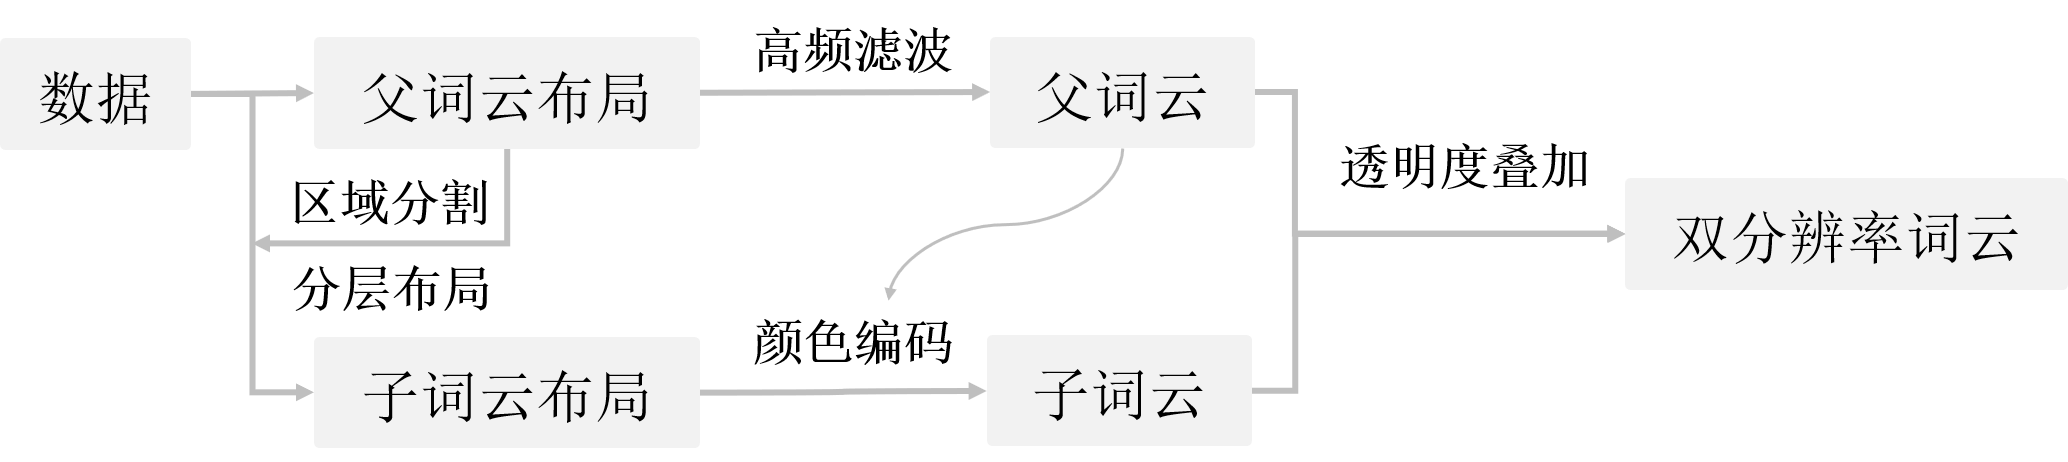
\includegraphics[width=\textwidth]{figures/pipeline.png}
	\caption{多分辨词云生成流程。}
	\label{fig:pipeline}
\end{figure}
\vspace{-1.2cm}

\section{数据}
双分辨率词云的基本数据模型可对应于二分图(见图~\ref{fig:data_model}),父级文本(如关键词,以下简称为父文本)与子级本文(如上下文,以下简称为子文本)之间存在层级的关系或语义上的关联。图中的每一个结点均具有字符串型文本属性和数值型的权重或词频属性(C2)。为了减少数据存储的冗余,使数据简洁而结构明晰,我们选择使用两个序列作为双分辨率词云的表示,分别对应于父文本和子文本,而关联信息编码在父文本各项中。
\begin{figure}[htbp]
	\centering
	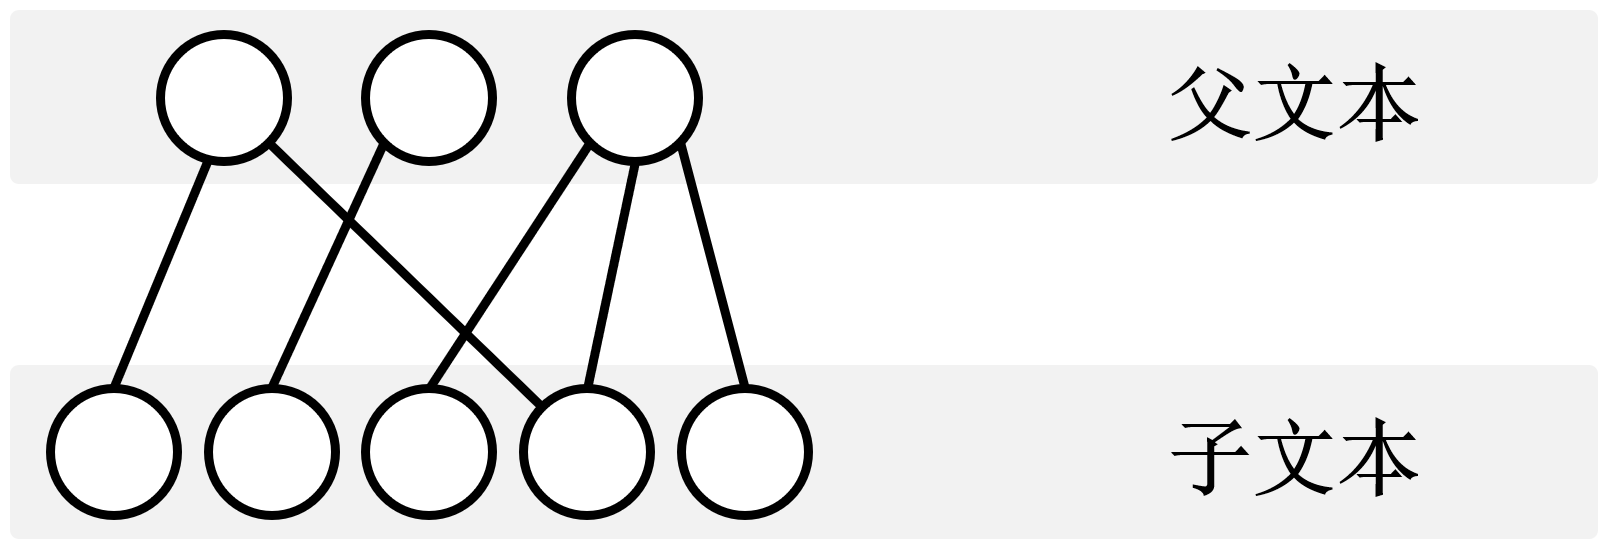
\includegraphics[width=0.6\textwidth]{figures/data_model.png}
	\caption{双分辨率词云数据模型。}
	\label{fig:data_model}
\end{figure}


使用\texttt{YAML}语言,双分辨率词云所对应的数据模型可形式化描述如下。需要注意的是,这里父文本与子文本的权重已归一化。在常见的词云算法中,归一化一般为词频直接除以最大值,亦有取对数或开平方后采用最小-最大归一的方法以降低极端值对整体的影响。

\begin{lstlisting}[language=yaml, caption=数据模型]
# %(*根对象*)
type: object
fileds:
	# %(*contexts域:序列类型,每个对象对应一个上下文*)
	contexts:
		type: sequence
		fields:
			#%(*context域:子文本,上下文*)
			context: { type: string }
			#%(*weight域:子文本权重*)
			weight: { type: number, min: 0, max: 1 }
	# %(*keywords域:序列类型,每个对象对应一个关键词*)
	keywords:
		type: sequence
		fields:
			# %(*keyword域: 父文本,关键词*)
			keyword: { type: string }
			# %(*weight域:关键词权重*)
			weight: { type: number, min: 0, max:1 }
			# %(*contexts域:集合类型,对应的子文本序列号*)
			context:
				type: set
				fields:
					# %(*contextID域:子文本序列号*)
					contextId: { type: number }
\end{lstlisting}

我们选用了《全唐诗》作为探索布局策略的基础数据,提取二字词中词频最高的$30$词作为父文本,对应的诗句(逗号或句号为分句符)作为子文本,并整理为以上数据模型所规定的格式进行尝试。其中,父文本的权重对应于其词频,而子文本的权重对应于该诗句作者在《全唐诗》中被收录的作品数量,在一定程度上通过作者的产量反映诗句的知名度。最终效果可查看图~\ref{fig:tang_poet}。

\section{布局算法}
\label{sec:layout}
我们依次确定父文本词云与子文本词云的位置。其中,父词云由已有词云算法给出,子词云则在对应父元素位置与字形的限制下布局。
\subsection{基础布局}
抽象而言,词云的布局算法就是在给定画布尺寸$w\times h$(长$\times$高)与词集合$\{w_i\}$及其对应字号后$\{s_i\}$,确定每个词在画布上的位置$\{(x_i,\  y_i)\}$,满足在该布局方案下按照给定字号与字体渲染出的词与词之间互不相交即可。

常见的词云算法在第2.3节已有概述,由于它们对不同的分析展示任务各有优势,我们选择在生成双分辨率词云的过程中保留词云布局算法的自由度,用户可根据不同的需求灵活选用适当的布局算法或自定义父词云位置。以下展示了一种最为简单的词云布局算法的伪代码,其主要思想是逐个确定位置,在备选区域中随机选择。
 \begin{algorithm}[htb]
	\caption{适用于轮廓限制的贪心词云布局算法}
	\label{alg:basic_layout}
	\begin{algorithmic}[1]
		\Require
		词云字体$font$;词云对应的文本有序列表$\{(word_i, size_i)\}$,包括文字$word$与字号$size$,顺序为字号由大到小,相同字号按照文字长度由大到小;轮廓限制$Mask$(一般情况下为空白)与其最小外接矩形规格$W\times H$
		\Ensure
		词云布局方案$P$
		\State 基于轮廓限制构建一个二值矩阵$M$,标记各离散像素点是否为空。对每一个词$i$计算最小邻接矩形$(w_i, h_i)$
		\State 创建位置集合$P=\{\}$
		\Repeat 对有序列表中的每一个词$i$
			\Repeat 从中心$(W/2, H/2)$开始,沿螺旋线扫描$M$上的像素点$(x-w_i/2,y-h_i/2)$
			\If {\textbf{} 若$(x-w_i/2,y-h_i/2)$与$(x+w_i/2, y+h_i/2)$为对角所张成的水平矩形区域全部为空}
			\State 向位置映射$P$添加$(word_i, size_i, x, y)$元组。
			\State 以字体$font$及字号$size_i$在画布上渲染文字$word_i$,更新$M$
			\EndIf
		\Until{$M$上不存在可放置词云的区域}
		\Until{$i$循环完毕}

	\end{algorithmic}
\end{algorithm}

\subsection{子文本布局}

\paragraph{区域分割}
根据设计选择C4,子词云应布局在父词云的邻域内。我们在得到父词云的基本布局后,还需进一步确定子词云可占据的位置。从另一个角度来说,就是要对对图像进行区域划分,使得每个区域两两不交,能够基本覆盖父词云并尽可能地利用上空白的位置。


\begin{figure}[htbp]
	\centering
	
\includegraphics[width=\textwidth]{figures/expand.png}
	\caption{基于父文本布局的子文本区域分割算法示意图。左:原始父词云及其外接矩形,根据是否存在重叠得到各边扩张(绿)/收缩(红)的初始设定。右:经过逐步迭代后得到稳定的分割结果。}
	\label{fig:expand_alg}
\end{figure}

如图~\ref{fig:expand_alg}所示,我们的区域分割采用了一种基于迭代的策略。首先,从已知的父词云外接矩形出发,根据其四边是否与其他外接矩形相交判断其移动的方向---(1)若存在相交情况,则需要向内收缩,直至不存在交叠。(2)若不存在相交,则向外扩张,直至下一次遇到边界或产生相交。在接下来的每次迭代中,各个矩形的四边均向外或向内移动一个像素,除非其已满足停止的要求。记整个画布规格为$W\times H$,每一个词均对应于左上角坐标为$(x_0, y_0)$、右下角坐标为$(x_1, y_1)$的外接矩形,图~\ref{fig:collide_rule}左侧列举了在每一次迭代中需要对坐标对进行监测的情况以及边界的限制。按照定位坐标的相对位置,可将产生重叠的情况进一步分为边角重叠与区域包含与被包含三个状态。

所有区域满足终止条件时,能够严格保证每一个区域不交。但是,此时空白的地方有可能尚未被充分地利用。为此,我们再次对结果进行扫描,使用贪心的策略,依次对每个矩形区域的四边进行舒张。当伸展方向上不包含其他矩形时直接言延伸到画布边界;而当某些矩形存在于伸展方向上时,则选取距离待考察矩形最近的区域作为伸展的限制(见图~\ref{fig:collide_rule}右侧)。为了避免某些区域由于循环顺序优势伸展过多,我们将四个方位放于循环体外部。

\begin{figure}[htbp]
	\centering
	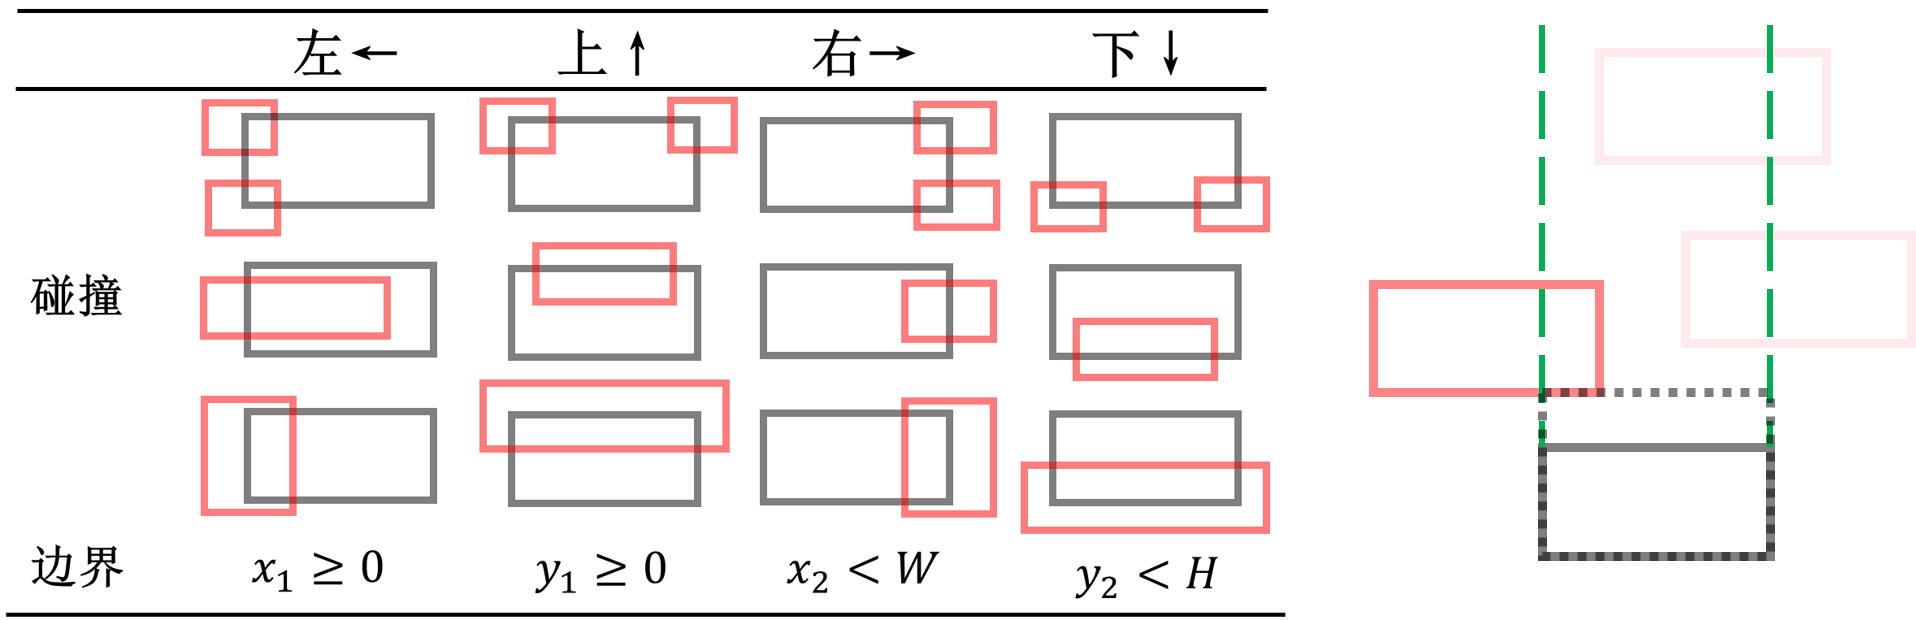
\includegraphics[width=\textwidth]{figures/collide_rule.png}
	\caption{左:子文本区域动态收缩/增长的监测规则与边界条件。黑色与红色矩形分别对应判断词云主体与相关区域。右:基于贪心策略的区域伸展策略。当黑色矩形需要向上伸展时,考察其上部在水平方向与其产生交叠的矩形区域,并基于距离最近矩形限制进行伸展。}
	\label{fig:collide_rule}
\end{figure}

\paragraph{分步布局}
获得子词云在画布上所对应的区域后,我们进一步考虑子词云的布局策略。若单纯随机布局,子词云与父词云之间会出现遮挡,不利于用户对文本的识别(P2.3)。为了充分利用可行区域(P2.1),我们在父词云实际所占区域的基础上,将子词云是否与其相交分为内外两层。内层子词云以父词云的轮廓作为边界,完全嵌套在父词云内部。而对于外层子词云,由于我们希望能稍加突出父词云的字形,我们使用父词云膨胀后取反的轮廓作为其布局的约束(见图~\ref{fig:sublayout})。
\begin{figure}[htbp]
	\centering
	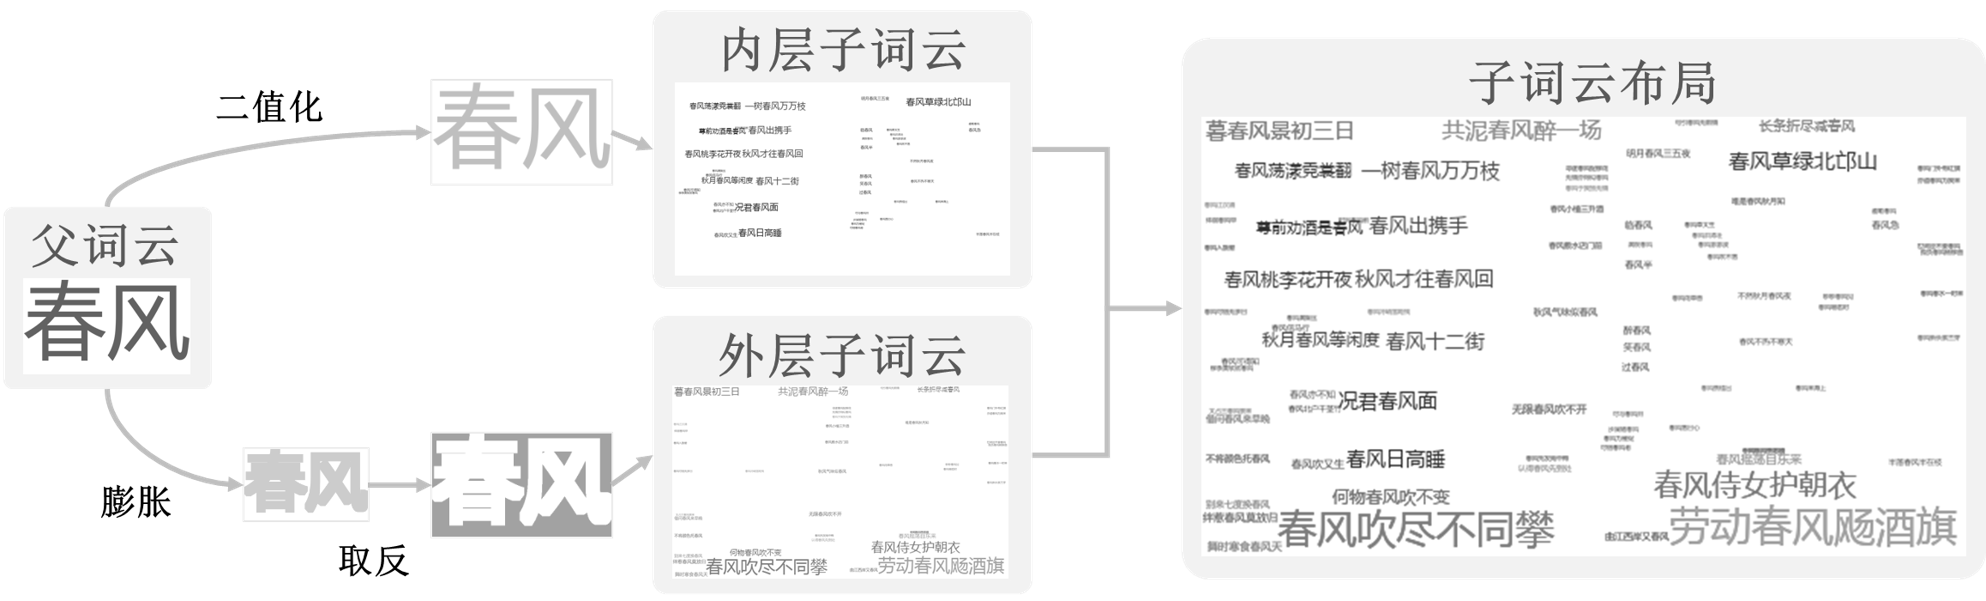
\includegraphics[width=\textwidth]{figures/sublayout.png}
	\caption{子词云分布布局的流程。首先以父文本构造布局约束,得到内层词云。再通过膨胀父文本结构后求反得到外层词云的布局约束,由此获得内层词云。}
	\label{fig:sublayout}
\end{figure}

膨胀的作用是一种常见的形态学处理方法,其作用是使二值图像中的物体沿轮廓向外扩大。设结构元$A$和集合$B$是$\mathbb{Z}^2$中的集合,则$A$对$B$的膨胀定义为
\begin{equation*}
A \oplus B = \{z|(\hat{B}_{z})\cap A = \varnothing\}.
\end{equation*}
此处我们设定结构元为以字符笔触宽度为边长的正方形,以此维护字体的原有形态。

\subsection{算法加速}
大屏上的双分辨率词云布局中最主要的问题就是分辨率过大,计算复杂。无论是使用何种算法,其复杂度都与画布尺寸相关,全屏情况即对应屏幕分辨率。由于无法避免检测词语位置是否重叠,基本上所有算法均需要对图像进行扫描,逐像素确定合适位置;而对于基于物理模拟的迭代算法如力导向布局,其计算更是代价高昂。因此,尽管以上的布局策略理论上可行,但在实际针对大屏的计算中,我们仍有一定的优化空间,提升算法效率。

首先,父文本词云的精确计算是不必要的。我们注意到,父文本词云具有相当大的字号,在远处浏览父词云的效果与在近处浏览常规词云的效果类似。换而言之,大屏上的父词云实际可视为整体放大的常规词云。因此,我们可以对父词云进行适当的全局放缩,在更小的画布上计算对应小字号词云的布局,再相应地映射到原有的大屏上,做一个简单的近似。

全局等比放缩系数$k$与父文本最小字号$m$有关。在设计选择的讨论中,我们已经确定父文本字号阈值设为$64$是合适的,而考虑到由于字号为离散整数,过度的放缩会限制词云字号的表示空间,也会产生过度失真的现象(见图~\ref{fig:font_size}),因此我们设定$16$像素为缩放后的最小字号,即$k = 64/16=4$。
\begin{figure}[htbp]
	\centering
	
\includegraphics[width=0.8\textwidth]{figures/font_size.png}
	\caption{不同分辨率下的文字``好'',从左至右由10\texttt{px}至22\texttt{px}。分辨率越低,字形失真越严重。}
	\label{fig:font_size}
\end{figure}

例如,对一个由4$\times$3个4K显示屏所组成的大型显示设备,其具有$w_1\times h_1 = 15360\times6480$的分辨率。我们通过缩放,基于$w_2\times h_2 = 3840\times 1620$的画布尺寸得到每个词的基础坐标$\{(x_i', y_i')\}$。那么,经过一个线性变化,即可得到在原始画布上的布局坐标估计值:
\begin{equation*}
\begin{pmatrix}
x_i\\
y_i
\end{pmatrix}
 =  k\begin{pmatrix}
 x_i'-w_2/2\\
 y_i'-h_2/2
 \end{pmatrix}
 +\begin{pmatrix}
w_1/2\\
 h_1/2
 \end{pmatrix} .
\end{equation*}

其次,区域分割亦可在放缩后的画布上进行,减少搜索的空间。相关定位点的坐标转换可参考上式的横纵坐标转换。

最后,子词云布局算法可数据并行。由于在分割区域时已保证各子词云位置无重叠,因此各父文本对应的子文本词云的计算是完全独立的,可充分利用大型显示设备的GPU资源等来进行并行化计算,加速双分辨率词云生成的过程。

\section{混合图像}
我们在混合父词云与子词云时主要考虑了频域滤波以及词语颜色编码两个层面,以产生双分辨率的效果,同时保持父子词云在视觉上既相互关联又互不干扰。
\subsection{词云融合}
双分辨率词云的关键在于使人们在不同的距离下关注到不同层次的词云。参考Olivia等人~\supercite{Olivia2006}的多分辨率图像生成算法,我们同样采用先过滤父文本词云的高频分量,再通过透明度叠加的方法混合上下两个图层的方法来得到最终的结果(见图~\ref{fig:blend})。

\begin{figure}[htbp]
	\centering
	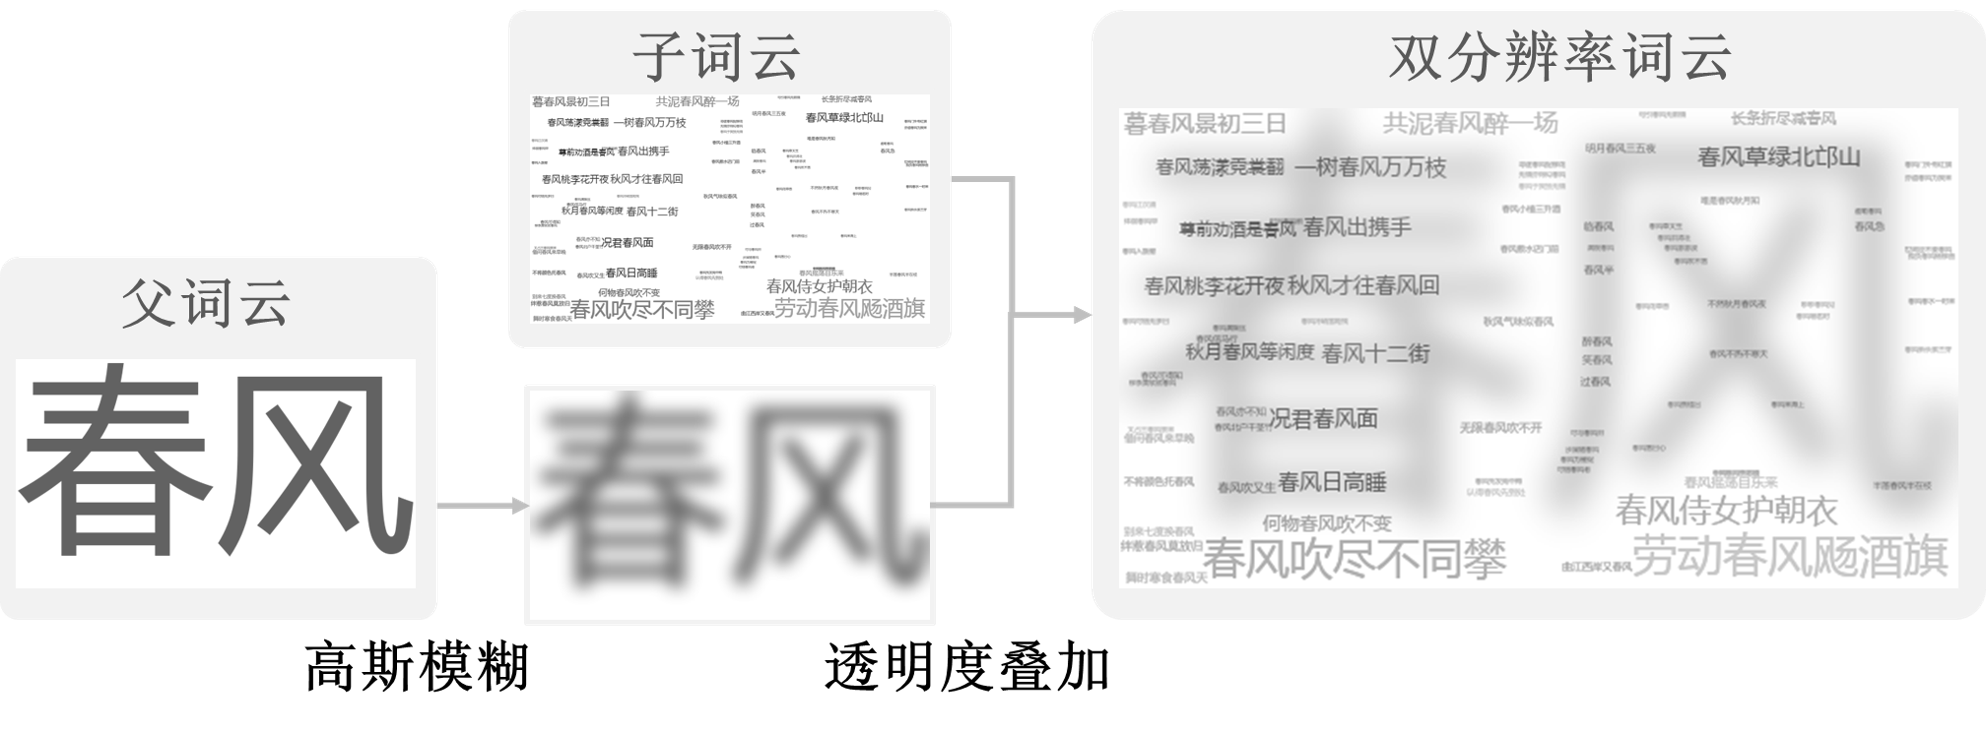
\includegraphics[width=\textwidth]{figures/blend.png}
	\caption{词云融合的流程图:保留父文本词云的高频分量,与子文本词云通过透明度互相叠加。}
	\label{fig:blend}
\end{figure}

由于子文本在双分辨率词云的设计中本就具有较小的字号,人们只有凑近屏幕至适宜阅读距离才能辨别,而滤波会影响其字形,因此我们不对其空间频域进行特殊处理。而对于字号较大的父文本,人们是从远处浏览,无需保留边界的细节即可辨认,且滤波后能够降低其对识别子词云产生的干扰,所以有必要过滤其高频分量。

简记在上一节所述布局算法得到的父文本词云为$I_1$,子文本词云为$I_2$。我们使用高斯滤波器对$I_1$进行卷积。一个标准的高斯函数$G(x,y)$的表达式为
\begin{equation*}
G(x,y) = \frac{1}{2\pi \sigma^2}e^{-\frac{x^2+y^2}{2\sigma^2}},
\end{equation*}
其中$\sigma$表示其标准差。一个高斯卷积核就是以核中心为原点的经过和归一化的离散高斯函数。
设$I_1$的最小字号为$s_{min} = \min_{i} s_i$,则我们限定高斯核$Ker(G)$的大小为$k^2 = ceil(\frac{s_{min}}{25})^2$。
\begin{equation*}
I_1' = I_1 \otimes Ker_k(G).
\end{equation*}
\begin{equation*}
I_2' = I_2.
\end{equation*}
$k$分母上的常数$25$是我们通过类似图~\ref{fig:font_size}的实验确定的,在常见的一些字体中,当分辨率$r$逐渐变大,对应字符比特图上的笔触宽度约为$ceil(\frac{r}{25})$。我们在全局使用与最小词云笔触大小一致的卷积核以防止字形剧变,影响识别。

经过$\alpha\in [0,1]\cap \mathbb{R}$的透明度叠加,最终得到的图像$I$可表示为
\begin{equation*}
I = \alpha I_1' + (1-\alpha)I_2'.
\end{equation*}


\subsection{颜色编码}

沿用设计选择C5,我们随机为父词云赋色,在此基础上对子词云添加扰动。但是,为了更加符合人的认知规律,我们选择在LCH色彩空间中进行相应的数值处理。

人是通过视网膜上分布的视杆细胞与视锥细胞来感知光线的,分别对应低亮度与高亮度的情况。Opponent-Process理论~\supercite{hurvich1957opponent}认为,大脑将感光细胞做感知到的光波处理为了三个通道——亮度、红绿与蓝黄通道。以此为理论指导,国际照明委员会定义了LAB色彩空间以模拟人的感知,经笛卡尔坐标系转换为圆柱坐标系后得到LCH色彩空间(见图~\ref{fig:color_rationale})。尽管彩色图片多以RGBA(分别对应红、绿、蓝、透明度)三个通道来编码一个像素所对应的颜色,使用RGB编码形式有利于计算机上的数字图像处理,但无论是基于RGB编码,亦或是可视化中常用的HSV/HSL编码,通过线性插值得到的渐变色并不能比拟于在HCL空间中所具有的渐变色依感知均匀分布的特性。
\begin{figure}[htbp]
	\centering
	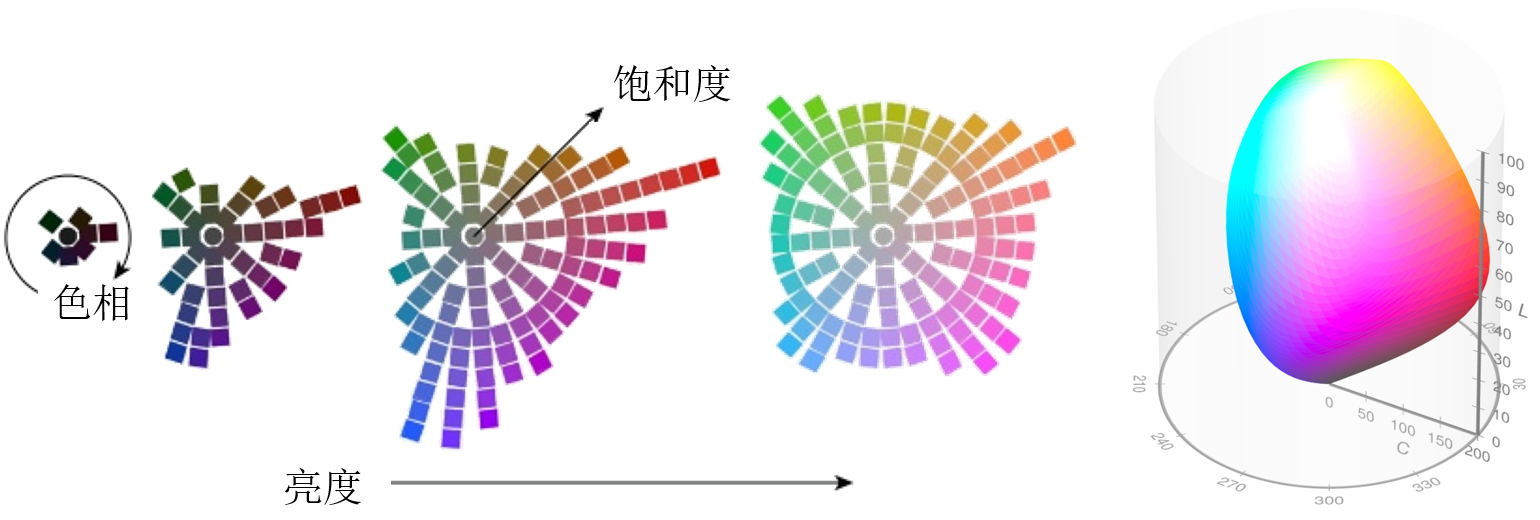
\includegraphics[width=0.9\textwidth]{figures/color_spec.png}
	\caption{色彩空间。左:不同亮度下人眼所能感知到的颜色示意(图源:NASA Earth Observatory\protect\footnotemark,标记经笔者翻译)。右:LCH色彩空间,分别对应亮度L、色度/饱和度C、与色相H(图源:维基百科\protect\footnotemark)。}
	\label{fig:color_rationale}
\end{figure}

\footnotetext{Subtleties of Color. Robert Simon. \url{https://earthobservatory.nasa.gov/blogs/elegantfigures/2013/08/05/subtleties-of-color-part-1-of-6/}}

\footnotetext{HCL color space. \url{https://en.wikipedia.org/wiki/HCL_color_space}}

在现有的普通词云布局算法中,颜色往往是独立于布局的,仅起到区分词语的作用。此时,这些算法会忽略透明度通道,直接随机取色或根据用户指定的一个配色方案在RGB空间中进行插值。对于具有语义聚类关系的词云,词云的色系将不同的类分别开,有时直接统一为同一颜色。而在双分辨词云中,经过一系列的测试与对比,我们设定了颜色编码规则如下,数值范围参考图~\ref{fig:color_rationale}右侧的色彩空间示意:

\begin{table}[htbp]
		 \caption{双分辨率词云色彩编码规则}
		 \label{tab:color_rule}
	\begin{tabular}{llll}

		\toprule
		&\multicolumn{1}{c}{父词云} & \multicolumn{1}{c}{相交子词云} & \multicolumn{1}{c}{不交子词云} \\
		\midrule
		亮度$L$ & 中等范围[$40,\  60$]    &   低亮度范围[$20,\  40$]     &    高亮度范围 [$60,\  80$]   \\
		色度$C$ &   中高色度范围 [$150,\  170$]  & 中色度范围[$120, \ 150$]     &  高色度范围 [$160,\  180$]       \\
		色相$H$ &  随机选择   &  父词云邻域 ±$10$°     &       父词云邻域  ±$10$°\\
		\bottomrule
	\end{tabular}
\vspace{-0.2cm}
\end{table}
在这一规则下,父词云区域与外部的子词云区域在亮度上具有较大的差异,但共享相同的色系,保证了在远处巨大的父词云清晰可辨(P2.3),并保留了父子词云的关联性。而在父词云的内部,同一色系但饱和度与亮度略低的子词云能够保证其不会完全混入父词云中,并能够强调父词云的字形。色彩的亮度实际上可以在背景色的基础上通过透明度来调节。但是,由于上下层词云混合时涉及到了基于透明度通道的图片叠加,为了减少不同参数对最终结果的关联性,我们在此并不考虑透明度。对于这样的规则,$\alpha$在$0.3\sim 0.5$的范围较为适宜(见图~\ref{fig:alpha_comparison})。
\vspace{-0.3cm}
\begin{figure}[htbp]
	\centering
	
\includegraphics[width=\textwidth]{figures/alpha_comparison.png}
	\caption{不同$\alpha$值下的多分辨率词云效果。在表~\ref{tab:color_rule}的规则下,0.3至0.5为宜。}
	\label{fig:alpha_comparison}
\end{figure}
\vspace{-0.2cm}

图~\ref{fig:color_comparison}对比了在RGB编码下的随机扰动与基于上述LCH空间中的扰动策略。可以观察到,尽管由于透明度叠加的原因,靠近屏幕时两种方法对应的子词云均清晰可辨;但当我们远离屏幕,LCH编码策略下外层词云总体偏亮的色彩能让我们更为轻松地辨认出父词云的字,而相对而言,RGB随机编码产生的图片稍显噪音过多。
\vspace{-0.1cm}
\begin{figure}[htbp]
	\centering
	
\includegraphics[width=\textwidth]{figures/color_comparison.png}
	\vspace{-0.5cm}
	\caption{子词云颜色编码策略对比。左:基于RGB空间的扰动。右:基于LCH空间的扰动。}
		\vspace{-0.5cm}
	\label{fig:color_comparison}
\end{figure}

	    \chapter{案例分析}
借助第四章描述的多分辨率词云生成方法,我们收集了几例不同性质的数据并生成相应的双分辨率词云,结合真实案例探讨这一可视化形式的参数调整及其有效性。

\section{文学作品}
《全唐诗》是清康熙四十五年由曹寅、彭定求、沈立曾、杨中讷等人奉敕编纂而成,共收录唐代诗人$2,529$人的诗作$42,863$首。我们选定高频双子词作为父文本,其字号直接对应于词频;而子词云则对应运用了该词的诗句。考虑到由于不同的诗在传诵程度上有所区别,而人们自然地对自己所熟知的诗感到亲近,为了增强该双分辨率词云的趣味性,我们假设诗人所收录作品数与其影响力有一定关联,故将其作为子词云的权重,来反映诗句可能的的流行度。

图~\ref{fig:tang_poet}展示了$28$个高频词所对应的部分上下文。可以观察到,《全唐诗》中带有负面情绪的词语偏多,如``不得''、``寂寞''、``惆怅''等,正应了``悲愤出诗人''的古话。而气象相关的词语为最常见的意向,如``明月''、``春风''、``秋风''、``白日''、``白云'',所谓寓情于景,大部分相关诗句虽关乎景,但其怅惘与忧思跃然纸上。

这一数据是\textbf{子文本基数大}的典型案例。由于在词云中,字号已预先指定,而布局中常用的贪心算法会因为布局区域的限制忽略掉重权重较小的词。案例图片展示的是对纸面规格设定较为适宜的词云,在$30cm\sim40cm$的普通阅读距离下即可同时观察双层词云,父词云远至$2m$外依然可辨,文本较为丰富,颇具代表性。但是,这也造成每个子文本区域的平均空间较少,能够放置的词云有限。此外,由于父词云笔触较细,有相当一部分父词云的内部区域未能被子词云填充。一个更好的选择是利用上大型显示设备的高分辨率特性来展示更多的数据,为数据提供全貌。


\section{社交媒体}
我们收集了美国总统唐纳德·约翰·特朗普(Donald J. Trump)自2020年一月一日至2020年五月十五日在社交平台Twitter上的原创发言记录\footnote{\url{https://twitter.com/realDonaldTrump}},共计$1852$条,平均每日约$13$条。我们以高频词语作为父文本,使用点赞数与转发数之和作为父文本的权重,以此反映该词的常用程度以及相关推文受到的关注。

在一般的词云中,关键词往往都非常精炼,从不会超过一行。但是,在双分辨率词云中,有可能存在父文本所对应的上下文或其他类型的子文本文字内容过长的情况,此时若依然维持一字排开会极大降低文本的易读性,距离较近时甚至需要观众移动以完整阅读。因此,在\textbf{子文本内容较长}的情况下,应对文本适当分行,控制近处视图内的文字。我们设置一行的宽度为最大$50$字符,使长句变为文本块。为避免出现两个文段交错布局的现象(参考图~\ref{fig:trump}),我们对算法1进行了适当的调整,将整个文本块视为一个整体,在更新二值矩阵时填充其最小外接矩形而非逐字渲染。

我们分别在普通桌面显示屏规格(图~\ref{fig:trump})和墙面规格(图~\ref{fig:wall})的设定下生成了特朗普推特的双分辨率词云。我们大致可从父文本内容中的名词了解到近半年以来,特朗普的推文多有关总统事务、民主党派、美国、伊朗、就业、新闻等等。而作为形容词的``Fake''使我们不明所以。进一步查看相关推文,我们发现它几乎完全以``FAKE NEWS''的形式出现,指责新闻报道失实,言辞间情绪激动,但并未给出明证与理由,正文末尾多附以超链接。从语言风格来看,特朗普似乎倾向于使用通俗易懂的词汇,且大量使用字母大写和感叹号,特别是对短短几字的推文。``Great''是词频最高的,推文中多次提到``Make America great again''的宣言,其他情况多表示对人事物的赞扬。

尽管《全唐诗》是在小空间下布局,但由于其子文本简短,整体空间利用率较高,疏密得当。但对于具有大块文字的推特数据而言,其在普通桌面显示屏下的效果欠佳。绝大部分父文本及其内部未能为子文本提供布局空间,画面稍显凌乱。这一问题在大屏设定下有所改善。在换用粗笔触字体并提高父子词云字号的差异后,更多空间得到填充,总体布局较为均匀。此外,得益于我们的高频滤波策略,内层子词云与外层子词云之间不存在太强的割裂感,颇为和谐。


\section{双层主题}

2020年5月22日,在第十三届全国人民代表大会第三次会议上,国务院总理李克强发表了《政府工作报告》\footnote{\url{http://www.gov.cn/zhuanti/2020lhzfgzbg}},重点提及了深化改革、扩大内需、脱贫攻坚、对外开放、保障改善民生与政府建设六点。我们以此为线索,人工梳理了发言稿中这六个主题下的子话题,将其可视化。此处相同层次文本的权重具有一定随机性,大致上相同,字号没有特定的指向性。

这一数据属于\textbf{子文本数据有限}的情况。因为父词云字号需要足够大,这会造成子词云可布局空间过大,从而使子词云过于稀疏,不利于集中地观察。此时,我们允许子文本重复出现,得到图~\ref{fig:gov}。这种方式尽最大可能地填满了所有空隙,保证了远处视图的美观。同时,我们设置画布为较小的规格,以避免词语重复过多。

\bigbreak

%\section{小结}
%在对以上数据的分析中,我们对不同规格的画布以及不同双层文本性质下的双分辨率词云进行了讨论,进一步明确了不同设定下的
%\begin{itemize}
%	\item \textbf{}
%\end{itemize}


\begin{figure}[htbp]
	\centering
	
\includegraphics[width=\textwidth]{figures/tang.png}
	\caption{纸面规格:《全唐诗》高频双子词云。}
	\label{fig:tang_poet}
\end{figure}


\begin{figure}[htbp]
	\centering
	
\includegraphics[width=\textwidth]{figures/trump.png}
	\caption{普通显示器规格:特朗普推特发言。}
	\label{fig:trump}
\end{figure}

\begin{figure}[htbp]
	\centering
		
\includegraphics[width=\textwidth]{figures/trump_crop.png}\\
		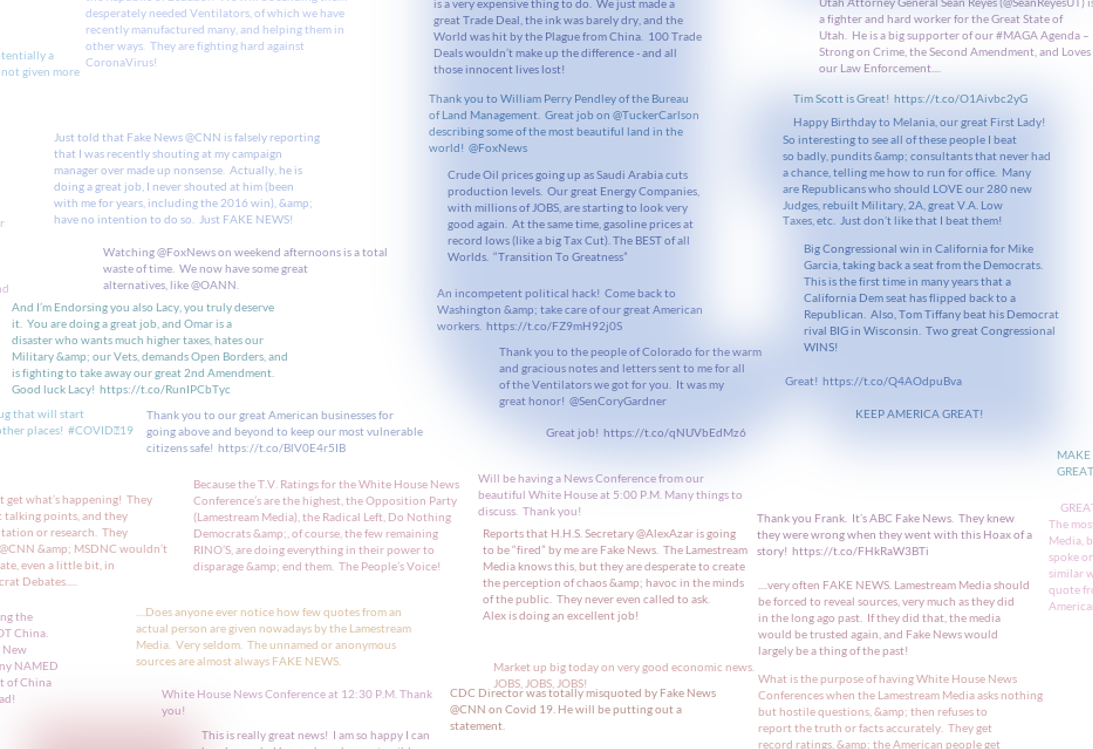
\includegraphics[width=\textwidth]{figures/trump_small.png}

	\caption{墙面规格:特朗普推特发言——概览及细节。}
		\label{fig:wall}

\end{figure}

\begin{figure}[htbp]
	\centering
	
\includegraphics[height=0.95\textheight]{figures/gov_paper.png}
	\caption{纸面规格:2020年政府工作报告。}
	\label{fig:gov}
\end{figure}

	\chapter{双分辨率词云创制系统}
\label{sec:system}
双分辨率词云是一种任务驱动型的基础可视化,可应用于相当广泛的文本数据。尽管它可以在上一章算法的基础上被独立开发实现,但由于它是一种新颖的可视化方法,且所涉及的参数较多,新接触的人群难以理解参数与最终效果的关联,且尚无完备的优化准则来指导机器自动生成,因此不利于创作者与分析人员的了解与利用。为此,我们设计开发了一套基于用户-服务器模型的交互创制系统,~\toolname{},以支持用户对双分辨率词云的便捷创制。

\section{设计要求}
基于在设计双分辨率词云可视化的迭代过程中所积累的一些经验以及对现有的在线词云创建系统的参考,我们总结出了以下几项对双分辨率词云创制系统的设计要求,以方便用户快速生成双分辨率词云,并在一定程度上控制最终的效果。

\begin{enumerate}[leftmargin=*]
	\renewcommand{\labelenumi}{\textbf{D\theenumi.}}
	\renewcommand{\labelenumii}{\textbf{D\theenumi.\arabic{enumii}}}
	\item \textbf{提供灵活的数据处理功能}:由于双分辨率词云适用于探索式分析任务(T1)和数据分享任务(T2),因此创制系统也应相应地对数据格式有更灵活的支持,为具有不同需求的用户提供服务。
	\begin{enumerate}
		\item \textbf{纯文本语料库}---对毫无先验知识的纯文本,用户可直接上传,系统在简单处理后可视化其高频词及对应语句或文短以提供具有语境的概览,帮助用户找到数据中感兴趣的内容,挖掘数据背后的洞见。
		\item \textbf{格式化文本}---对数据已具备一定了解的用户亦可指定双层词云各自的具体内容,构建映射关系,展示相应的内容,促进交流。在这种情境下,系统应不再局限于简单的文本挖掘,支持用户自定义所需要可视化的内容。
	\end{enumerate}
	\item \textbf{支持对效果的调整}:在数据分享任务(T2)和寓教于乐任务(T3)中,可视化的最终效果需要符合设计者一定的心理预期,支持设计者对布局及格式的调整。
		\begin{enumerate}
		\item \textbf{参数推荐}---过于灵活的参数设置容易使可视化经验较少的用户茫然无措,而本研究所提出的双分辨率词云更是一种全新的方法,我们尚未充分地认识到参数与效果之间的对应关系。因此,我们需要在交互的过程中为用户提供更多的指引,基于固定的在不影响用户与系统交互的效率的前提下,尽可能地缩小用户需要探索的参数空间。
		\item \textbf{反馈效果}---及时反馈参数所对应的效果,避免让用户通过不断生成双分辨率词云的低效方式来调试。
		\item \textbf{自定义}---用户可具体指定各词语的可视化参数,如父文本词云(或与子文本词云)的布局位置或赋色方案。
	\end{enumerate}
\end{enumerate}

\section{系统概览}
\toolname{}是一个轻型的网站,由四个页面组成:主页、创制页面、画廊及说明页,采用前后端分离的客户-服务器模式。

\subsection{界面}
\subsection{交互逻辑}



\section{前后端交互}
\subsection{数据上传}
本节简要介绍该系统所支持的数据格式与布局参数接口。在下一章里,我们将通过几个具体的例子,说明该设定如何能够方便用户运用双分辨率词云可视化。
\paragraph	{\textbf{格式化文本}}
在前一章的数据模型设计下,\toolname{}以\texttt{json}作为双分辨率词云的的底层数据格式,并接收用户上传的符合规范的\texttt{json}数据(格式规范如下所示),以适应于更广泛的数据类型(D1.2)。这是一种独立于程序的数据交换语言,具有以下优点。
\begin{itemize}
	\item \textbf{易读性强}---它的层次结构清晰而简洁,易于理解。
	\item \textbf{普及性高}---\texttt{json}是ECMAScript®语言规范的标准之一,受几乎所有编程语言的支持,用户可在简单的数据预处理后生成相应文件。
	\item \textbf{适合网络上的数据交换}---在客户端与服务器端数据传输的过程中针对\texttt{json}型数据存在特定的压缩技术,能够节省带宽。
\end{itemize}

在此基础上,我们给予用户定制可视化的空间,允许他们指定父级词云的位置与颜色(D2.3)。

\begin{lstlisting}[language=json, caption=\texttt{json}上传数据格式规范,父级词云的位置与颜色域可为空]
{
	"keyword_list": {
		keyword_id: {
			"word": keyword_string,
			"weight": weight_of_word,
			"contexts": [
				context_id
			],
			"position": [x, y],
			"color": color_string
	},
	"context_list": [
		context_id: {
			"context": context_string,
			"weight": weight_of_context
		}
	]
}
\end{lstlisting}

\paragraph {\textbf{纯文本}}
在常见的词云创制网站,如Wordle~\footnote{\url{http://www.wordle.net}}和Word Art~\footnote{\url{https://wordart.com}}中,用户通过复制粘贴文本或指定文字来源网页超链接的方式来指定可视化的内容,限定使用\texttt{UTF-8}编码。注意到它们对于电子书、预印本等常见语料库的支持不足,我们还在系统内额外增添了\texttt{pdf}和\texttt{txt}格式的文件处理机制(D1.1),将他们转化为字符串。


\paragraph{\textbf{布局参数}}

\subsection{数据处理}
对于用户所上传的无任何先验知识的纯文本,系统默认将词频高的关键词作为父词云,其所在句子作为子词云。为了进一步确定用户所关心的细节程度,我们需要用户输入句子的分隔符,默认为句号、分号、感叹号与问号。

中文、日文、泰文等本文的一大特色在于,它们的句段中短语或词组不存在天然的分隔符。而由于语言的歧义性、词库有限等诸多难题,如何准确分词至今仍是热门的研究方向。为此,系统使用了性能较为良好的``结巴分词''\footnote{\url{https://github.com/fxsjy/jieba}}进行了分词操作以提取关键词。

\subsection{参数推荐}




\section{系统实现}
本研究所实现的双分辨率词云创制系统的\texttt{HTML5}网站在前端部分使用了轻量级的\texttt{Vue} 框架生成动态页面,以\texttt{JavaScript}语言协调用户与系统的交互,包括数据上传、参数输入、输入完整性检验与推荐,以及生成图像预览与下载。而后端部分则是基于\texttt{Flask}框架响应前端请求,对于自定义数据进行相应的处理,并根据参数返回生成的词云。后端所用程序语言为\texttt{Python},单独开发了双分辨率词云的类库,提供函数接口,在词云布局的迭代算法中使用了\texttt{Cython}以进行加速。

\draft{采访系统使用感受。}

    \chapter{讨论与展望}
\section{优势}
\begin{itemize}
	\item \textbf{展示层次文本数据}双分辨率词云是一种适用于具有双层关系的文本可视化方法,能够在现有词云概览的基础上进一步提供更多关联的信息,有利于观者更为准确地理解文本数据。
	\item \textbf{支持大规模数据}
	\item \textbf{具有艺术性}。经过基于LCH空间的色彩扰动,双分辨率词云
\end{itemize}


尽管在上文中没有提及,
\section{局限与挑战}
\begin{itemize}
	\item \textbf{纯静态展示,交互空间尚未探索。}
	\item \textbf{非实时加载,需要一定的计算时间,对大型显示设备所耗时更长。}
	\item \textbf{用户定制空间不足。}相较于成熟的词云生成软件,我们的创制系统目前对,我们通过一些参数
	\item \textbf{用户测试。}
\end{itemize}

\section{未来工作与潜在研究机会}
\begin{itemize}
	\item \textbf{探索双分辨率词云的交互空间。}
	\item \textbf{自动与交互之间。}利用Pops Out现象。
	\item \textbf{强化色彩编码。}在基于大屏的双分辨率词云的使用场景中,子
\end{itemize}

   \chapter{结论}


	% 正文中的附录部分。
	\appendix
	% 排版参考文献列表。bibintoc 选项使“参考文献”出现在目录中;
	% 如果同时要使参考文献列表参与章节编号,可将“bibintoc”改为“bibnumbered”。
	\printbibliography[heading=bibintoc, title={参考文献}]
	% 各附录。
%	% Copyright (c) 2014,2016 Casper Ti. Vector
% Public domain.

\chapter{附件}
\pkuthssffaq % 中文测试文字。

% vim:ts=4:sw=4


	% 以下为正文之后的部分,默认不进行章节编号。
	\backmatter
	% 致谢。
	\chapter{本科期间的主要工作和成果}

\noindent 已接收论文
\begin{enumerate}
	\item \textbf{Liwenhan Xie}, James O'Donnell, Benjamin Bach, and Jean-Daniel Fekete. Interative Time-Series of Measures for Exploring Dynamic Networks. \emph{International Conference on Advanced Visual Interfaces}, Salerno, Italy, 2020.
	\item Can Liu, \textbf{Liwenhan Xie}, Yun Han, Datong Wei and Xiaoru Yuan. AutoCaption: An Approach to Generate Natural Language Description from Visualization Automatically. \emph{IEEE Pacific Visualization Symposium (Notes)}, Tianjin, China, 2020.
\end{enumerate}

\noindent 获奖作品/海报
\begin{enumerate}
	\item Shuai Chen, Sihang Li, \textbf{Liwenhan Xie}, Yi Zhong, Yun Han, and Xiaoru Yuan. EarthquakeAware: Visual Analytics for Understanding Human Impacts of Earthquakes from Social Media Data. \emph{IEEE Symposium on Visual Analytics Science and Technology (VAST Challenge)}, Vancouver, Canada, 2019. \textbf{Honorable Mention for Support for Analysis through Annotation and Context Award}.
	\item Can Liu, \textbf{Liwenhan Xie}, Yun Han, Datong Wei and Xiaoru Yuan. Auctomatic Caption Generation for SVG Charts. \emph{IEEE Pacific Visualization Symposium}, Bangkok, Thailand, 2019. \textbf{Honorable Mention for Best Poster Award}.
	\item Qi Ma, Chuangming Huang, \textbf{Liwenhan Xie}, Zhiyi Yin ,and Xiaoru Yuan.  Visual Analysis for Subgroups in a Dynamic Network. \emph{IEEE Symposium on Visual Analytics Science and Technology (VAST Challenge)}, Berlin, Germany, 2019. \textbf{Insights Generated Through the Use of a Custom Tool Award}.
	\item Lijing Lin, \textbf{Liwenhan Xie}, Zhuo Zhang, and Xiaoru Yuan. Visualizing Dynamic Networks of Long Sequences with Pixel Matrix Array. \emph{China Visualization and Visual Analytics Conference}, Sichuan, China, 2018. \textbf{Honorable Mention for Best Poster Award}.

\end{enumerate}

	% Copyright (c) 2014,2016 Casper Ti. Vector
% Public domain.

\chapter{致谢}
感谢袁晓如老师三年以来对我的启发与指导。也感谢香港科技大学的屈华民教授,爱丁堡大学的Benjamin Bach教授,巴黎综合理工大学的Emmanuel Pietriga教授以及法国自动化研究所的Jean-Daniel Fekete教授。他们是我在学术道路上的引路人,我从他们身上体会到了科研工作者应有的态度与担当。

感谢一路上所遇到的同侪,和一群热爱可视化的人一起成长是一种幸福。特别感谢从各方面带我熟悉科研的陈帅师兄、林丽静师姐、伍翱宇师兄和刘灿师兄;经常与我交流点子的李国政师兄;对深陷bug泥潭的我热心伸出援手的田敏师兄、魏大同师兄、吴聪师兄和林志贤师兄,以及曾不吝给予指点的陈思明师兄、刘子鹏师兄、陈玺师姐和俞博文师兄。

感谢我的室友陈思如、杨静仪、张佳雨和泛心桥数风事务所的伙伴们,和他们相处的时光洋溢着欢乐。也感谢这个园子提供的各种机遇与可能,还有总在第一时间予我慰藉的湖心岛老松树。

感谢我的父母及家人在各种意义上对我的支持。

感谢我的朋友潘薇宇、刘升雯、单婧怡、韦嘉睿、孙伟健、Mohammad Mahzoun、严加恩、符芬菊、林之韵、曾琳总是耐心聆听我排山倒海的碎嘴。

感谢校友Casper、solvethis提供的论文模板。

% vim:ts=4:sw=4

	% 原创性声明和使用授权说明。
	% Copyright (c) 2008-2009 solvethis
% Copyright (c) 2010-2017 Casper Ti. Vector
% All rights reserved.
%
% Redistribution and use in source and binary forms, with or without
% modification, are permitted provided that the following conditions are
% met:
%
% * Redistributions of source code must retain the above copyright notice,
%   this list of conditions and the following disclaimer.
% * Redistributions in binary form must reproduce the above copyright
%   notice, this list of conditions and the following disclaimer in the
%   documentation and/or other materials provided with the distribution.
% * Neither the name of Peking University nor the names of its contributors
%   may be used to endorse or promote products derived from this software
%   without specific prior written permission.
%
% THIS SOFTWARE IS PROVIDED BY THE COPYRIGHT HOLDERS AND CONTRIBUTORS "AS
% IS" AND ANY EXPRESS OR IMPLIED WARRANTIES, INCLUDING, BUT NOT LIMITED TO,
% THE IMPLIED WARRANTIES OF MERCHANTABILITY AND FITNESS FOR A PARTICULAR
% PURPOSE ARE DISCLAIMED. IN NO EVENT SHALL THE COPYRIGHT HOLDER OR
% CONTRIBUTORS BE LIABLE FOR ANY DIRECT, INDIRECT, INCIDENTAL, SPECIAL,
% EXEMPLARY, OR CONSEQUENTIAL DAMAGES (INCLUDING, BUT NOT LIMITED TO,
% PROCUREMENT OF SUBSTITUTE GOODS OR SERVICES; LOSS OF USE, DATA, OR
% PROFITS; OR BUSINESS INTERRUPTION) HOWEVER CAUSED AND ON ANY THEORY OF
% LIABILITY, WHETHER IN CONTRACT, STRICT LIABILITY, OR TORT (INCLUDING
% NEGLIGENCE OR OTHERWISE) ARISING IN ANY WAY OUT OF THE USE OF THIS
% SOFTWARE, EVEN IF ADVISED OF THE POSSIBILITY OF SUCH DAMAGE.

{
	\ctexset{section = {
		format+ = {\centering}, beforeskip = {40bp}, afterskip = {15bp}
	}}

	% 学校书面要求本页面不要页码,但在给出的 Word 模版中又有页码且编入了目录。
	% 此处以 Word 模版为实际标准进行设定。
	\specialchap{北京大学学位论文原创性声明和使用授权说明}
	\mbox{}\vspace*{-3em}
	\section*{原创性声明}

	本人郑重声明:
	所呈交的学位论文,是本人在导师的指导下,独立进行研究工作所取得的成果。
	除文中已经注明引用的内容外,
	本论文不含任何其他个人或集体已经发表或撰写过的作品或成果。
	对本文的研究做出重要贡献的个人和集体,均已在文中以明确方式标明。
	本声明的法律结果由本人承担。
	\vskip 1em
	\rightline{%
		论文作者签名:\hspace{5em}%
		日期:\hspace{2em}年\hspace{2em}月\hspace{2em}日%
	}

	\section*{%
		学位论文使用授权说明\\[-0.33em]
		\textmd{\zihao{5}(必须装订在提交学校图书馆的印刷本)}%
	}

	本人完全了解北京大学关于收集、保存、使用学位论文的规定,即:
	\begin{itemize}
		\item 按照学校要求提交学位论文的印刷本和电子版本;
		\item 学校有权保存学位论文的印刷本和电子版,
			并提供目录检索与阅览服务,在校园网上提供服务;
		\item 学校可以采用影印、缩印、数字化或其它复制手段保存论文;
		\item 因某种特殊原因须要延迟发布学位论文电子版,
			授权学校在 $\Box$\nobreakspace{}一年 /
			$\Box$\nobreakspace{}两年 /
			$\Box$\nobreakspace{}三年以后在校园网上全文发布。
	\end{itemize}
	\centerline{(保密论文在解密后遵守此规定)}
	\vskip 1em
	\rightline{%
		论文作者签名:\hspace{5em}导师签名:\hspace{5em}%
		日期:\hspace{2em}年\hspace{2em}月\hspace{2em}日%
	}

	% 若须排版二维码,请将二维码图片重命名为“barcode”,
	% 转为合适的图片格式,并放在当前目录下,然后去掉下面 2 行的注释。
	%\vfill\noindent
	%\includegraphics[height = 5em]{barcode}
}

% vim:ts=4:sw=4

\end{document}

% vim:ts=4:sw=4
